\def\GraphicsFolder{chapters/superconducting-instability/pictures}
\chapter{Superconducting instability}\label{chap:mft-sc-instability}

In this chapter the HF methods introduced in Sec.~\ref{sec:sketch-hf-method} are applied to the SC phase. We study a translationally invariant superconductor, which breaks the conservation of total charge. Analytic calculations will lead us to various effects: bare bands renormalisation, anisotropic Cooper pairing and nematicity. Our description of the SC phase is closely related to the BCS solution for pure $s$-wave superconductivity.

As for previous phases, this chapter is divided in three parts. First, analysis of the SC phase symmetries based on the discussion of Chap.~\ref{chap:ehm-symmetries}, and implementation of HF methods. Second, search for theoretical constraints on the self-consistent solution. Third, numeric results.

\section{The SC phase and its symmetries}\label{sec:sc-phase-theory}

As for antiferromagnetism, superconductivity can establish in a variety of ways. We deal with the simplest realisation. In Sec.~\ref{subsec:ehm-sym-break} we anticipated that the SC phase is described by the two SSBs
\[
\begin{aligned}
	\mathrm{U}^z(1) &\SSB 0 \\
	\mathrm{C}_4 &\SSB \mathrm{C}_2
\end{aligned}
\]
Translational invariance is unbroken. Then electronic density needs to be uniform across all sites, similarly to the normal phase discussed in Chap.~\ref{chap:normal-phase}. Non-uniform density distributions are inconsistent with translational invariance in both directions. We have, then
\begin{equation}\label{eq:sc-density-ansatz}
	\ev{\hat n_{\mathbf{r}\sigma}} = n
\end{equation}
which is identical to Eq.~\eqref{eq:normal-density-ansatz} for the normal phase.

Recall Tabs.~\ref{tab:HU-sel-rules} and \ref{tab:HV-sel-rules}, collecting the selection rules for the local repulsion $\hat H_U$ and the non-local attraction $\hat H_V$. From Eqns.~\eqref{eq:mft-HU}, \eqref{eq:mft-HV} for the SC phase we need to account for the following contractions:
\[
\begin{aligned}
	&\hat H_U 
	&&\text{Hartree and Cooper contractions} \\
	&\hat H_V \text{ (o.s. sector)}
	&&\text{Hartree and Cooper contractions} \\
	&\hat H_V \text{ (s.s. sector)}
	&&\text{Hartree and Fock contractions} \\
\end{aligned}	
\]
We anticipate their roles in Tab.~\ref{tab:sc-RWCs}.

\begin{table}[t]
	\centering
	\begin{tabular}{c c c l}
		\textbf{Operator} & \textbf{Sector} & \textbf{RWCs} & \textbf{Net effect} \\
		\midrule
		\multirow{2}{*}{$\hat H_U$} && Hartree & $\mu$ shift by $-nU$ \\
		&& Cooper & Isotropic pairing in singlet channel \\
		\midrule
		\multirow{4}{*}{$\hat H_V$} & \multirow{2}{*}{o.s.} & Hartree & $\mu$ shift by $nzV$ \\
		&& Cooper & Anisotropic pairing in singlet and triplet channels \\[0.5em]
		& \multirow{2}{*}{s.s.} & Hartree & $\mu$ shift by $nzV$ \\
		&& Fock & Band renormalisation and resymmetrisation \\
		\midrule
	\end{tabular}
	\caption{Relevant Wick's contractions and net effect in the SC phase. This RWCs table is more structured than Tabs.~\ref{tab:normal-RWCs} and \ref{tab:af-RWCs}.}
	\label{tab:sc-RWCs}
\end{table}

The SSB of $\mathrm{U}^z(1)$ allows for EVs like $\langle \hat c^\dagger \hat c^\dagger \rangle$ to be non-zero. This leads to the formation of Cooper pairs. These are composite quantum objects with a specific spin-spatial structure. Consider the generic Cooper fluctuation
\[
	\big\langle
	\hat c_{i\sigma}^\dagger \hat c_{j\overline{\sigma}}^\dagger
	\big\rangle
	\qq{with $i,j$ nearest neighbours}
\]
We work in o.s. sector because we know from Tab.~\ref{tab:HV-sel-rules} that the s.s. sector is prohibited. From basic Quantum Mechanics we know the summation rules of the spin algebra $\mathfrak{su}(2)$,
\[
	\frac 1 2 \otimes \frac 1 2 = 0 \oplus 1
\]
The two pairing channels are, at this level, the singlet channel associated to total spin $0$ and the triplet channel associated to total spin $1$. Now, when applying HF method to the quartic operators, we get the decomposition of Eq.~\eqref{eq:mft-V-decomposition}. We can impose to the approximated HF ground-state a particular spatial structure -- say, inversion symmetry or antisymmetry. This reflects in the requirement that Cooper pairs show the same spatial structure.

This gives a selection rule over Cooper pairings: if we work with inversion-symmetric structures -- say, $s^*$-wave or $d$-wave -- the pairing will take place in singlet channel, allowing us to eliminate the triplet pairing. Working with antisymmetric structures, inversely, we can eliminate the singlet channel. This concept is summarised in Tab.~\ref{tab:sc-pairings-symmetry-structures}.

\begin{table}
	\centering
	\begin{tabular}{c c}
		\textbf{Spatial structure} & \textbf{Pairing channel} \\
		\midrule
		Symmetric wave function & Singlet pairing \\
		Anti-symmetric wave function & Triplet pairing \\
		\midrule
	\end{tabular}
	\caption{Relation of the Cooper pairing channel with the wavefunction spatial symmetry (intended as the inversion $(x,y) \to (-x,-y)$).}
	\label{tab:sc-pairings-symmetry-structures}
\end{table}

We proceed as we did for the AF phase: in order to highlight the physical effects of $\hat H_V$, we first analyse the SC phase limitedly to the conventional HM. In next section we prove that BCS-like superconductivity is impossible at HF level on the pure HM, with just the local repulsion $\hat H_U$. It is the presence of the non-local attraction that enables Cooper pairing mechanism. Before starting, let
\begin{align}
	\hat n_{\mathbf{k}\sigma} &\equiv \hat c_{\mathbf{k}\sigma}^\dagger \hat c_{\mathbf{k}\sigma} \label{eq:sc-ehm-n-def} \\
	\hat \phi_\mathbf{k} &\equiv \hat c_{-\mathbf{k}\downarrow} \hat c_{\mathbf{k}\uparrow}\label{eq:sc-ehm-phi-def}
\end{align}
where $\hat n_{\mathbf{k}\sigma}$ was defined as for the AF phase, in Eq.~\eqref{eq:af-ehm-n-def}. The HF approximation in reciprocal space to the EHM will be written in terms of these operators.

\section{Local effects: (impossibility of) superconductivity in the HM}\label{sec:sc-local}

Let us start from the local effects. Following Tab.~\ref{tab:HU-sel-rules} and Eqns.~\eqref{eq:mft-HU}, \eqref{eq:mft-HV}, we know the local repulsion decomposes in Hartree and Cooper channels,
\[
\begin{aligned}
	\hat H_U &= U \sum_{\mathbf{r}\in\mathcal{L}} \hat n_{\mathbf{r}\uparrow} \hat n_{\mathbf{r}\downarrow} \label{eq:mft-HU} \\
	&\simeq U \sum_{\mathbf{r}\in\mathcal{L}} \Big(
	\hat c_{\mathbf{r}\uparrow}^\dagger \hat c_{\mathbf{r}\uparrow} \big\langle \hat c_{\mathbf{r}\downarrow}^\dagger \hat c_{\mathbf{r}\downarrow} \big\rangle + \big\langle \hat c_{\mathbf{r}\uparrow}^\dagger \hat c_{\mathbf{r}\uparrow} \big\rangle \hat c_{\mathbf{r}\downarrow}^\dagger \hat c_{\mathbf{r}\downarrow} - \big\langle \hat c_{\mathbf{r}\uparrow}^\dagger \hat c_{\mathbf{r}\uparrow} \big\rangle  \big\langle \hat c_{\mathbf{r}\downarrow}^\dagger \hat c_{\mathbf{r}\downarrow} \big\rangle &&(\text{Hartree}) \\
	&\phantom{\simeq \sum_{{\mathbf{r}\uparrow}\neq{\mathbf{r}\downarrow}} V_{{\mathbf{r}\uparrow}{\mathbf{r}\downarrow}}}
	+ \hat c_{\mathbf{r}\uparrow}^\dagger \hat c_{\mathbf{r}\downarrow}^\dagger \big\langle \hat c_{\mathbf{r}\downarrow} \hat c_{\mathbf{r}\uparrow} \big\rangle + \big\langle \hat c_{\mathbf{r}\uparrow}^\dagger \hat c_{\mathbf{r}\downarrow}^\dagger \big\rangle \hat c_{\mathbf{r}\downarrow} \hat c_{\mathbf{r}\uparrow} - \big\langle \hat c_{\mathbf{r}\uparrow}^\dagger \hat c_{\mathbf{r}\downarrow}^\dagger \big\rangle  \big\langle \hat c_{\mathbf{r}\downarrow} \hat c_{\mathbf{r}\uparrow} \big\rangle
	\Big) &&(\text{Cooper})
\end{aligned}
\]
In next sections we deal with each channel separately.

\subsection{Local Hartree channel in the SC phase: analytic derivation}\label{subsec:sc-l-hartree-analytic}

For the Hartree channel, being the density uniform across sites, we can re-use the entirety of Sec.~\ref{subsec:normal-hartree-analytic} for the normal phase. Substituting Eq.~\eqref{eq:sc-density-ansatz}, we get the approximation of Eq.~\eqref{eq:normal-HU-approx},
\begin{equation}\label{eq:sc-HU-approx}
	\hat H_U \simeq nU \times \hat N - E_{\mathrm{H}/U}^{(\mathrm{SC})} + \text{(Cooper channel)}
\end{equation}
thus chemical potential renormalization $\tilde{\mu} \to \mu - nU$ is present also in the SC phase.

\subsection{Local Hartree contraction energy}\label{subsec:sc-l-hartree-energy}

As for the section above, we use the result of Sec.~\ref{subsec:normal-hartree-energy} for the normal phase. From Eq.~\eqref{eq:normal-hartree-U-contraction-energy}
\begin{equation}\label{eq:sc-hartree-U-contraction-energy}
	E_{\mathrm{H}/U}^{(\mathrm{SC})} = L_x L_y \times n^2 U
\end{equation}
For a locally repulsive model, the Hartree channel contributes negatively to ground state energy. Indeed, contraction energy is subtracted from the hamiltonian. We now move to the Cooper channel.

\subsection{Local Cooper channel in the SC phase: analytic derivation}\label{subsec:sc-l-cooper-analytic}

We move to reciprocal space, through the transformation of Eq.~\eqref{eq:HU-fourier}. Consider the Cooper channel of Eq.~\eqref{eq:mft-HU}. In reciprocal space we get:
\begin{multline}
	\hat H_U \simeq \text{(Hartree channel)} + \frac{U}{L_x L_y}
	\sum_{\mathbf{K}, \mathbf{k}, \mathbf{k}'} \Big[
	\big\langle
	\hat c_{\mathbf{K}+\mathbf{k} \uparrow}^\dagger \hat c_{\mathbf{K}-\mathbf{k} \downarrow}^\dagger
	\big\rangle \hat c_{\mathbf{K}-\mathbf{k}' \downarrow} \hat c_{\mathbf{K}+\mathbf{k}' \uparrow} \\
	+ \hat c_{\mathbf{K}+\mathbf{k} \uparrow}^\dagger \hat c_{\mathbf{K}-\mathbf{k} \downarrow}^\dagger \big\langle
	\hat c_{\mathbf{K}-\mathbf{k}' \downarrow} \hat c_{\mathbf{K}+\mathbf{k}' \uparrow} 
	\big\rangle - \big\langle
	\hat c_{\mathbf{K}+\mathbf{k} \uparrow}^\dagger \hat c_{\mathbf{K}-\mathbf{k} \downarrow}^\dagger
	\big\rangle \big\langle 
	\hat c_{\mathbf{K}-\mathbf{k}' \downarrow} \hat c_{\mathbf{K}+\mathbf{k}' \uparrow}
	\big\rangle
	\Big] \label{eq:sc-mft-HU}
\end{multline}
We are not breaking translational invariance, thus only Cooper fluctuations with net zero total momentum are allowed. This means only $\mathbf{K}=\mathbf{0}$ contributes. Let us prove this: consider the EV of the Cooper pair
\[
	\big\langle \hat c_{\mathbf{k}_1\uparrow}^\dagger \hat c_{\mathbf{k}_2\downarrow}^\dagger \big\rangle
\]
for two momenta $\mathbf{k}_1$, $\mathbf{k}_2$. Moving to real space via an $\mathcal{F}$-transform, we get
\[
	\big\langle \hat c_{\mathbf{k}_1\uparrow}^\dagger \hat c_{\mathbf{k}_2\downarrow}^\dagger \big\rangle \Feq \frac{1}{L_x L_y} \sum_{\mathbf{r}_1 \in \mathcal{L}} \sum_{\mathbf{r}_2 \in \mathcal{L}} e^{-i \left(\mathbf{k}_1 \cdot \mathbf{r}_1 + \mathbf{k}_2 \cdot \mathbf{r}_2\right)} \big\langle \hat c_{\mathbf{r}_1\uparrow}^\dagger \hat c_{\mathbf{r}_2\downarrow}^\dagger \big\rangle
\]
where we used the convention of Eq.~\eqref{eq:fourier-convention}. Let now $\mathbf{r}_1 \to \mathbf{r}$ and $\mathbf{r}_2 \to \Delta \mathbf{r}$. Translational invariance implies that
\[
	g(\Delta \mathbf{r}) = \big\langle \hat c_{\mathbf{r}\uparrow}^\dagger \hat c_{\mathbf{r}+\Delta\mathbf{r}\downarrow}^\dagger \big\rangle
\]
is independent of $\mathbf{r}$. Thus we have:
\[
\begin{aligned}
	\big\langle \hat c_{\mathbf{k}_1\uparrow}^\dagger \hat c_{\mathbf{k}_2\downarrow}^\dagger \big\rangle &\Feq \sum_{\Delta\mathbf{r} \in \mathcal{L}} e^{-i \mathbf{k}_2 \cdot \Delta\mathbf{r}} g(\Delta \mathbf{r}) \frac{1}{L_x L_y} \sum_{\mathbf{r} \in \mathcal{L}} e^{-i \left(\mathbf{k}_1 + \mathbf{k}_2\right) \cdot \mathbf{r}} \\
	&= \sum_{\Delta\mathbf{r} \in \mathcal{L}} e^{-i \mathbf{k}_2 \cdot \Delta\mathbf{r}} g(\Delta \mathbf{r}) \delta_{\mathbf{k}_1=\mathbf{k}_2}
\end{aligned}
\]
where we used the identity of Eq.~\eqref{eq:ehm-delta}. Then the above EV vanishes for $\mathbf{k}_1\neq\mathbf{k}_2$. Getting back to Eq.~\eqref{eq:sc-mft-HU}, this proves that only pairs at null total momentum can have nonzero EVs.

Let now $w_\mathbf{k}$ be the EV of $\phi_\mathbf{k}^\dagger$, and $w^{(s)}$ its $s$-wave projection:
\begin{align}
	w_\mathbf{k} &\equiv \big\langle
	\phi_\mathbf{k}^\dagger
	\big\rangle \label{eq:sc-wq-def} \\
	w^{(s)} &\equiv \frac{1}{L_x L_y} \sum_{\mathbf{q}\in\mathrm{BZ}} w_\mathbf{k} \label{eq:sc-hm-ws-self-consistency}
\end{align}
Eq.~\eqref{eq:sc-mft-HU} reduces to
\begin{equation}\label{eq:sc-HU-<phi>-phi}
	\hat H_U \simeq \text{(Hartree channel)} + \frac{U}{L_x L_y} \sum_{\mathbf{k},\mathbf{k}'} \left[
	\big\langle
	\hat \phi_\mathbf{k}^\dagger
	\big\rangle \hat \phi_{\mathbf{k}'} + 
	\hat \phi_\mathbf{k}^\dagger \big\langle
	\hat \phi_{\mathbf{k}'}
	\big\rangle
	\right] - E_{\mathrm{C}/U}^{(\mathrm{SC})}
\end{equation}
being $E_{\mathrm{C}/U}^{(\mathrm{SC})}$ the HM Cooper contraction energy, written explicitly in Sec.~\ref{subsec:sc-l-cooper-energy}. Let now
\begin{equation}\label{eq:sc-Delta^s}
	\Delta^{(s)} \equiv -U w^{(s)}
\end{equation}
This is the $s$-wave component of the gap function. Note that, in general, $\Delta^{(s)} \in \mathbb{C}$. However, we can always choose $\Delta^{(s)}$ as purely real. This is due to the fact that the hamiltonian is gauge-invariant, then it suffices to apply the gauge map of Eq.~\eqref{eq:gauge-symmetry} to the fermionic operators with
\[
	\eta \equiv \frac{\arg \Delta^{(s)}}{2}
\]
to obtain $\Delta^{(s)} \in \mathbb{R}$. For the sake of generality, we proceed with $\Delta^{(s)} \in \mathbb{C}$. Although this choice gives no advantage now, we implement it anyway in order to derive the most general form of the equations that follow. This is useful for the generalisation to the EHM.

In the end, we reduce $\hat H_U$ from Eq.~\eqref{eq:sc-HU-<phi>-phi} to
\begin{equation}\label{eq:sc-HU-gap-phi}
	\hat H_U \simeq \text{(Hartree channel)} - \sum_{\mathbf{k}\in\mathrm{BZ}} \left[
	\Delta^{(s)} \hat \phi_\mathbf{k} + 
	\Delta^{(s)*} \hat \phi_\mathbf{k}^\dagger
	\right] - E_{\mathrm{C}/U}^{(\mathrm{SC})}
\end{equation}
This last decomposition resembles Eq.~\eqref{eq:af-HU-gap-psi}, obtained for the AF phase in the Hartree channel.

\subsection{Local Cooper contraction energy}\label{subsec:sc-l-cooper-energy}

The Cooper contraction energy in the Cooper channel is given by:
\begin{align}
	E_{\mathrm{C}/U}^{(\mathrm{SC})} &\equiv \frac{U}{L_x L_y} \sum_{\mathbf{k}\mathbf{k}'} \big\langle
	\hat \phi_\mathbf{k}^\dagger
	\big\rangle \big\langle
	\hat \phi_{\mathbf{k}'}
	\big\rangle \nonumber \\
	&= L_x L_y \times U \big| w^{(s)} \big|^2 \label{eq:sc-cooper-U-contraction-energy}
\end{align}
As for the Hartree channel, also the Cooper channel contributes negatively to ground-state energy.

\subsection{Superconductivity in the HM}\label{subsec:sc-hm}

We proceed here as we did for the AF phase in Sec.~\ref{subsec:af-hm}. We start by giving a matrix representation of the approximated hamiltonian, then map it to a pseudospin problem and finally specify how to diagonalise it to retrieve its ground state.

\paragraph{Matrix representation.}

Collecting the results of the above paragraphs, we obtain the quadratic approximation to the Hubbard hamiltonian in the SC phase,
\begin{multline}
	\hat H_t + \hat H_U \simeq \sum_{\mathbf{k} \in \mathrm{BZ}} \sum_\sigma \epsilon_{\mathbf{k}\sigma}
	\hat c_{\mathbf{k}\sigma}^\dagger \hat c_{\mathbf{k}\sigma} \\
	- \sum_{\mathbf{k}\in\mathrm{BZ}} \left[
	\Delta^{(s)} \hat \phi_\mathbf{k} + 
	\Delta^{(s)*} \hat \phi_\mathbf{k}^\dagger
	\right] + nU \times \hat N - \left[
	E_{\mathrm{H}/U}^{(\mathrm{SC})} + E_{\mathrm{C}/U}^{(\mathrm{SC})}
	\right]
	\label{eq:sc-hm-mft-h} 
\end{multline}
We define the shifted bare bands:
\[
	\xi_\mathbf{k} \equiv \epsilon_\mathbf{k} - \tilde{\mu}
\]
Notice we are using the renormalised chemical potential. Due to inversion symmetry, it holds $\xi_\mathbf{k} = \xi_{-\mathbf{k}}$. Using Fermi anticommutation rules, the kinetic operator can be written as:
\[
\begin{aligned}
	\hat H_t - \tilde{\mu}\hat N &= \sum_\sigma \sum_{\mathbf{k} \in \mathrm{BZ}} \xi_{\mathbf{k}\sigma} \hat n_{\mathbf{k}\sigma} \\
	&= \sum_{\mathbf{k} \in \mathrm{BZ}} \left(
		\xi_\mathbf{k} \hat n_{\mathbf{k}\uparrow} + \xi_{-\mathbf{k}} \hat n_{-\mathbf{k}\downarrow} 
	\right) \\
	&= \sum_{\mathbf{k} \in \mathrm{BZ}} \xi_\mathbf{k} \left(
		 \hat c_{\mathbf{k}\uparrow}^\dagger \hat c_{\mathbf{k}\uparrow} - \hat c_{-\mathbf{k}\downarrow} \hat c_{-\mathbf{k}\downarrow}^\dagger + 1
	\right) \\
	&= \sum_{\mathbf{k} \in \mathrm{BZ}} \xi_\mathbf{k} \left(
		\hat c_{\mathbf{k}\uparrow}^\dagger \hat c_{\mathbf{k}\uparrow} - \hat c_{-\mathbf{k}\downarrow} \hat c_{-\mathbf{k}\downarrow}^\dagger
	\right) + E_\mathrm{a}^{(\mathrm{SC})}
\end{aligned}
\]
being $E_\mathrm{a}^{(\mathrm{SC})}$ the ``anticommutation energy''
\begin{equation}\label{eq:sc-anticommutation-energy}
	E_\mathrm{a}^{(\mathrm{SC})} \equiv \sum_{\mathbf{k}\in\mathrm{BZ}} \xi_\mathbf{k}
\end{equation}

In the end, the hamiltonian is approximated by:
\begin{multline*}
	\hat H_t + \hat H_U \simeq \sum_{\mathbf{k} \in \mathrm{BZ}} \epsilon_\mathbf{k}
	\left[
		\hat c_{\mathbf{k}\uparrow}^\dagger \hat c_{\mathbf{k}\uparrow}
		- \hat c_{\mathbf{k}\downarrow} \hat c_{\mathbf{k}\downarrow}^\dagger
	\right] + E_\mathrm{a}^{(\mathrm{SC})} \\
	- \sum_{\mathbf{q}\in\mathrm{BZ}} \left[
		\Delta^{(s)} \hat \phi_\mathbf{q} + 
		\Delta^{(s)*} \hat \phi_\mathbf{q}^\dagger
	\right] + nU \times \hat N - \left[
		E_{\mathrm{H}/U}^{(\mathrm{SC})} + E_{\mathrm{C}/U}^{(\mathrm{SC})}
	\right]
\end{multline*}
with $E_{\mathrm{H}/U}^{(\mathrm{SC})}$, $E_{\mathrm{C}/U}^{(\mathrm{SC})}$ the contraction energies arising from Hartree and Cooper channels, and $E_\mathrm{a}^{(\mathrm{SC})}$ the energy shift resulting from anticommutation rules, given respectively in Eqns.~\eqref{eq:sc-hartree-U-contraction-energy}, \eqref{eq:sc-cooper-U-contraction-energy}, and \eqref{eq:sc-anticommutation-energy}. We recognised the $s$-wave gap $\Delta^{(s)}$ from Eq.~\eqref{eq:sc-Delta^s}.

Let the Nambu spinor
\[
	\hat \Phi_\mathbf{k} \equiv \begin{bmatrix}
			\hat c_{\mathbf{k}\uparrow} \\
			\hat c_{-\mathbf{k}\downarrow}^\dagger
		\end{bmatrix}
\] 
The approximated hamiltonian can be written in matrix form as:
\[
	\hat H_t + \hat H_U - \mu \hat N \simeq \sum_{\mathbf{k} \in \mathrm{BZ}} \sum_\sigma \hat \Phi_\mathbf{k}^\dagger h_\mathbf{k} \hat \Phi_\mathbf{k} + E_\mathrm{a}^{(\mathrm{SC})} - \left[
		E_{\mathrm{H}/U}^{(\mathrm{SC})} + E_{\mathrm{C}/U}^{(\mathrm{SC})}
	\right]
\]
being
\[
	h_\mathbf{k} \equiv \begin{bmatrix}
		\xi_\mathbf{k} & -\Delta_\mathbf{k}^* \\
		-\Delta_\mathbf{k} & - \xi_\mathbf{k}
	\end{bmatrix}
	\qq{with}
	\xi_\mathbf{k} \equiv \epsilon_\mathbf{k} - \tilde{\mu}
\]
and $\Delta_\mathbf{k} = \Delta^{(s)}$. 

\paragraph{Pseudospin representation.}

The hamiltonian can be written equivalently as
\[
	h_\mathbf{k} = \xi_\mathbf{k} \tau^z - \Re\lbrace \Delta_\mathbf{k} \rbrace \tau^x - \Im\lbrace \Delta_\mathbf{k} \rbrace \tau^y
\]
Let now the pseudospin operator $\hat{\mathbf{s}}_\mathbf{k}$
\[
	\hat s_\mathbf{k}^\alpha \equiv \hat \Phi_\mathbf{k}^\dagger \tau^\alpha \hat \Phi_\mathbf{k}
	\qq{with}
	\hat{\mathbf{s}}_{\mathbf{k}\sigma} = \begin{bmatrix}
		\hat s_{\mathbf{k}\sigma}^x \\
		\hat s_{\mathbf{k}\sigma}^y \\
		\hat s_{\mathbf{k}\sigma}^z
	\end{bmatrix}
\]
and the pseudofield $\mathbf{b}_\mathbf{k}$:
\[
	\mathbf{b}_\mathbf{k} \equiv \begin{bmatrix}
		- \Re \lbrace \Delta_\mathbf{k} \rbrace \\ - \Im \lbrace \Delta_\mathbf{k} \rbrace \\ \xi_\mathbf{k} 
	\end{bmatrix}
\]
For a purely real gap, the pseudofield has no $y$ component. In general, different gauges rotate the pseudofield around the $z$ axis.

As was for the AF phase, these operators satisfy a $\mathfrak{su}(2)$ algebra up to an constant, irrelevant in the context of this discussion. They satisfy the identities:
\begin{align}
	\hat s_\mathbf{k}^x &= \hat \phi_\mathbf{k} + \hat \phi_\mathbf{k}^\dagger \label{eq:sc-hm-x-psi} \\
	\hat s_\mathbf{k}^y &= i \left(
	\hat \phi_\mathbf{k} - \hat \phi_\mathbf{k}^\dagger 
	\right) \label{eq:sc-hm-y-psi} \\
	\hat s_\mathbf{k}^z &= \hat n_{\mathbf{k}\uparrow} + \hat n_{\mathbf{k}\downarrow} - 1\label{eq:sc-hm-z-psi} 
\end{align}
We report the EVs related to these identities Tab.~\ref{tab:sc-pseudo-spin-map}.

\begin{table}
	\centering
	\begin{tabular}{c c}
		\textbf{EV} & \textbf{Meaning} \\
		\midrule
		$\ev{\hat s_\mathbf{k}^x}$ & $\ev{
			\hat \phi_\mathbf{k}
			+ \hat \phi_\mathbf{k}^\dagger
		}$ \\[0.7em]
		$\ev{\hat s_\mathbf{k}^y}$ & $i \ev{
			\hat \phi_\mathbf{k}
			- \hat \phi_\mathbf{k}^\dagger
		}$ \\[0.7em]
		$\ev{\hat s_\mathbf{k}^z}$ & $\ev{
			\hat n_{\mathbf{k}\uparrow}
			+ \hat n_{-\mathbf{k}\downarrow}
		} - 1$ \\
		\midrule
	\end{tabular}
	\caption{List of the various expectation values (EVs) of each pseudospin component and their meaning in terms of fermionic operators.}
	\label{tab:sc-pseudo-spin-map}
\end{table}

We express the approximated hamiltonian in pseudospin representation as:
\begin{equation}\label{eq:sc-hm-spin-h}
	\hat H_t + \hat H_U - \mu \hat N \simeq \sum_{\mathbf{k} \in \mathrm{BZ}} \mathbf{b}_\mathbf{k} \cdot \hat{\mathbf{s}}_\mathbf{k} + nU \hat N + E_\mathrm{a}^{(\mathrm{SC})} - \left[
		E_{\mathrm{H}/U}^{(\mathrm{SC})} + E_{\mathrm{C}/U}^{(\mathrm{SC})}
	\right]
\end{equation}
This operator is similar enough to the one found for the AF phase, in Eq.~\eqref{eq:af-hm-spin-h}. It describes a set of pseudospin subject to a uniform field. As for the AF phase, we define the Bogoliubov bands $E_\mathbf{k}$
\[
	E_\mathbf{k} \equiv \sqrt{\xi_\mathbf{k}^2 + \abs{\Delta_\mathbf{k}}^2}
\]
The key difference with the AF Bogoliubov bands of Eq.~\eqref{eq:af-bands} is that $E_\mathbf{k}$ now are functions of $\tilde{\mu}$, since $\xi_\mathbf{k}$ depends on the chemical potential. In other words, now the Bogoliubov bands depend on the shifted bands $\xi_\mathbf{k}$ instead of the bare bands $\epsilon_\mathbf{k}$.

Moreover, let us define the angles $\theta_\mathbf{k}$, $\zeta_\mathbf{k}$ as
\[
	\cos 2\theta_\mathbf{k} = \frac{\xi_\mathbf{k}}{E_\mathbf{k}}
	\qquad
	\sin 2\theta_\mathbf{k} \cos 2\zeta_\mathbf{k} = \frac{\Re\lbrace \Delta_\mathbf{k} \rbrace}{E_\mathbf{k}}
	\qquad
	\sin 2\theta_\mathbf{k} \sin 2\zeta_\mathbf{k} = \frac{\Im\lbrace \Delta_\mathbf{k} \rbrace}{E_\mathbf{k}}
\]
Note that choosing the gauge $\eta = \arg \Delta^{(s)}/2$ the imaginary part of the gap is zero, and this reflects in $2\zeta_\mathbf{k}=k \times 2\pi$ with $k \in \mathbb{Z}$.

\paragraph{Diagonalisation.}

For the SC phase, diagonalisation of the HF hamiltonian follows the same procedure as was for the AF phase. Indeed, the diagonalising matrix is given by
\begin{align}
	W_\mathbf{k} &\equiv e^{-i \theta_\mathbf{k} \tau^y} e^{-i \zeta_\mathbf{k} \tau^z} \nonumber \\
	&= \begin{bmatrix}
		\cos \theta_\mathbf{k} & - \sin \theta_\mathbf{k} \\
		\sin \theta_\mathbf{k} & \cos \theta_\mathbf{k}
	\end{bmatrix} \begin{bmatrix}
		e^{-i\zeta_\mathbf{k}} & \\ 
		& e^{i\zeta_\mathbf{k}}
	\end{bmatrix} \nonumber \\
	&= \begin{bmatrix}
		\cos \theta_\mathbf{k} e^{-i\zeta_\mathbf{k}} & - \sin \theta_\mathbf{k} e^{i\zeta_\mathbf{k}} \\
		\sin \theta_\mathbf{k} e^{-i\zeta_\mathbf{k}} & \cos \theta_\mathbf{k} e^{i\zeta_\mathbf{k}}
	\end{bmatrix} \label{eq:sc-hm-diagonalizer}
\end{align}
and the graphic procedure is the same of Fig.~\ref{fig:pseudo-magnetic-field-hm}, with $\epsilon \to \xi$. We get:
\begin{equation}\label{eq:sc-WhW+-hm}
	d_\mathbf{k} = W_\mathbf{k} h_\mathbf{k} W_\mathbf{k}^\dagger
	\qq{with}
	d_\mathbf{k} \equiv \begin{bmatrix}
		E_\mathbf{k} & \\
		& - E_\mathbf{k}
	\end{bmatrix}
\end{equation}

In the tilted frame we have the expression for the Nambu spinors:
\begin{equation}\label{eq:sc-Gamma=WPsi}
	\hat\Gamma_\mathbf{k} = W_\mathbf{k} \hat \Psi_\mathbf{k}
\end{equation}
Explicitly:
\begin{align}
	\hat\Gamma_\mathbf{k} &= \begin{bmatrix}
		\cos \theta_\mathbf{k} e^{-i\zeta_\mathbf{k}} & - \sin \theta_\mathbf{k} e^{i\zeta_\mathbf{k}} \\
		\sin \theta_\mathbf{k} e^{-i\zeta_\mathbf{k}} & \cos \theta_\mathbf{k} e^{i\zeta_\mathbf{k}}
	\end{bmatrix} \begin{bmatrix}
		\hat c_{\mathbf{k}\uparrow} \\
		\hat c_{-\mathbf{k}\downarrow}^\dagger 
	\end{bmatrix} \nonumber \\
	&= \begin{bmatrix}
		\cos \theta_\mathbf{k} e^{-i\zeta_\mathbf{k}} \hat c_{\mathbf{k}\uparrow} - \sin \theta_\mathbf{k} e^{i\zeta_\mathbf{k}} \hat c_{-\mathbf{k}\downarrow}^\dagger  \\
		\sin \theta_\mathbf{k} e^{-i\zeta_\mathbf{k}} \hat c_{\mathbf{k}\uparrow} + \cos \theta_\mathbf{k} e^{i\zeta_\mathbf{k}} \hat c_{-\mathbf{k}\downarrow}^\dagger
	\end{bmatrix} \equiv
	\begin{bmatrix}
		\hat \gamma_\mathbf{k}^{(+)} \\
		\hat \gamma_\mathbf{k}^{(-)} 
	\end{bmatrix} \label{eq:sc-Gamma=WPsi-explicit}
\end{align}
The new Fermionic operators describe a Fermi gas on distributed on two mirrored bands,
\[
	\hat H_t + \hat H_U - \tilde{\mu} \hat N \simeq \sum_{\mathbf{k} \in \mathrm{BZ}} \sum_\sigma E_\mathbf{k} \left(
	\hat \gamma_\mathbf{k}^{(+)\dagger} \hat \gamma_\mathbf{k}^{(+)} - \hat \gamma_\mathbf{k}^{(-)\dagger} \hat \gamma_\mathbf{k}^{(-)}
	\right) + (\cdots) 
\]
with $(\cdots)$ the various energy shifts.

\subsection{Features of the SC solution}\label{subsec:sc-features}

In this section we give some details about the HF solution for the translationally-invariant SC phase. We prove that in the conventional HM, with local repulsion $\hat H_U$, isotropic BCS-like superconductivity is forbidden. This serves as ground to motivate the passage to the EHM.

\paragraph{Pseudospin EVs.}

The EVs of pseudospin operators in the various directions are given by:
\[
\begin{aligned}
	\langle \hat \Psi_\mathbf{k}^\dagger \tau^x \hat \Psi_\mathbf{k} \rangle &= -\sin 2\theta_\mathbf{k} \cos 2\zeta_\mathbf{k} \langle \hat \Gamma_\mathbf{k}^\dagger \tau^z \hat \Gamma_\mathbf{k} \rangle \\
	\langle \hat \Psi_\mathbf{k}^\dagger \tau^y \hat \Psi_\mathbf{k} \rangle &= -\sin 2\theta_\mathbf{k} \sin 2\zeta_\mathbf{k} \langle \hat \Gamma_\mathbf{k}^\dagger \tau^z \hat \Gamma_\mathbf{k} \rangle  \\
	\langle \hat \Psi_\mathbf{k}^\dagger \tau^z \hat \Psi_\mathbf{k} \rangle &= \cos 2\theta_\mathbf{k} \langle \hat \Gamma_\mathbf{k}^\dagger \tau^z \hat \Gamma_\mathbf{k} \rangle
\end{aligned}
\]
In the tilted frame, the averaged $z$ projection of pseudospin is:
\begin{equation}\label{eq:sc-<z>}
	\langle \hat \Gamma_\mathbf{k}^\dagger \tau^z \hat \Gamma_\mathbf{k} \rangle =
	f\left(
	E_\mathbf{k};\beta,0
	\right) - f\left(
	-E_\mathbf{k};\beta,0
	\right)
\end{equation}
Compared with the respective relation for the AF phase, Eq.~\eqref{eq:af-<z>}, the main difference here is that the chemical potential inside the Fermi-Dirac distribution is set to zero. This is due to the fact that $\tilde{\mu}$ is already included in the renormalised bands $E_\mathbf{k}$. The approximated quadratic hamiltonian describes a gas of $\gamma$ fermions at null chemical potential.

Let us define the thermal factors:
\begin{equation}\label{eq:sc-Th}
	\mathrm{Th}_\mathbf{k}^{(\pm)}[\beta] \equiv 
	f\left(
	-E_\mathbf{k};\beta,0
	\right) \pm f\left(
	E_\mathbf{k};\beta,0
	\right)
\end{equation}
In the end we have the EVs:
\begin{align}
	\ev{\hat s_\mathbf{k}^x} &= \frac{\Re \lbrace \Delta_\mathbf{k} \rbrace}{E_\mathbf{k}} \mathrm{Th}_\mathbf{k}^{(-)}[\beta] \label{eq:sc-hm-sx}\\
	\ev{\hat s_\mathbf{k}^y} &= \frac{\Im \lbrace \Delta_\mathbf{k} \rbrace}{E_\mathbf{k}} \mathrm{Th}_\mathbf{k}^{(-)}[\beta] \label{eq:sc-hm-sy}\\
	\ev{\hat s_\mathbf{k}^z} &=  -\frac{\xi_\mathbf{k}}{E_\mathbf{k}}  \mathrm{Th}_\mathbf{k}^{(-)}[\beta] \label{eq:sc-hm-sz}
\end{align}
Note that, as is expressed in Tab.~\ref{tab:sc-pseudo-spin-map}, the $z$ component of the pseudospin is related to density, being $1+\ev{\hat s_\mathbf{k}^z} = \ev{\hat n_{\mathbf{k}\uparrow}	+ \hat n_{-\mathbf{k}\downarrow}}$.

\paragraph{$s$-wave gap self-consistency equation.}

Applying the HF method to the conventional HM in SC phase, we obtained just one HFP: $w^{(s)}$. Let us derive its self-consistency equation. First, let
\[
	\tau^\pm \equiv \frac{\tau^x \pm i \tau^y}{2}
\]
Recall Eq.~\eqref{eq:sc-hm-ws-self-consistency} and expand it, to obtain
\begin{align}
	w^{(s)} &= \frac{1}{L_x L_y} \sum_{\mathbf{k}\in\mathrm{BZ}} \big\langle
	\hat \phi_\mathbf{k}^\dagger
	\big\rangle \nonumber \\
	&= \frac{1}{L_x L_y} \sum_{\mathbf{k}\in\mathrm{BZ}} \big\langle
	\hat \Phi_\mathbf{k}^\dagger \tau^+ \hat \Phi_\mathbf{k}
	\big\rangle \nonumber \\
	&= \frac{1}{L_x L_y} \sum_{\mathbf{k}\in\mathrm{BZ}} \frac{	
		\ev{\hat s_\mathbf{k}^x} + i \ev{\hat s_\mathbf{k}^y}
	}{2} \nonumber \\
	&= \frac{1}{2 L_x L_y} \sum_{\mathbf{k}\in\mathrm{BZ}} \frac{\Delta_\mathbf{k}}{E_\mathbf{k}} \mathrm{Th}_\mathbf{k}^{(-)}[\beta] \label{eq:sc-hm-ws-self-consistency-2}
\end{align}
Last line is the explicit form of the self-consistency equation for $w^{(s)}$.

\paragraph{Impossibility of $s$-wave superconductivity.}

Let us define the critical $U$,
\begin{equation}\label{eq:sc-Uc}
	U_\mathrm{c}[\beta] \equiv \left[
	\frac{1}{2 L_x L_y} \sum_{\mathbf{k}\in\mathrm{BZ}} \frac{\mathrm{Th}_\mathbf{k}^{(-)}[\beta]}{E_\mathbf{k}}
	\right]^{-1}
\end{equation}
We call it ``critical'' because its value gives a sort of boundary for convergence. Indeed, as we show in App.~\ref{appendix:sc-g-opt}, for the SC phase in conventional HM, we are able to optimise parametrically the mixing parameter $g$ in order to ensure convergence, based on the ratio $U/U_\mathrm{c}[\beta]$. 

Let us show that superconductivity is not possible in the conventional HM with $U>0$. Eq.~\eqref{eq:sc-hm-ws-self-consistency-2} can be rewritten as:
\[
	w^{(s)} = -\frac{U}{U_\mathrm{c}[\beta]} w^{(s)}
\]
By construction $U_\mathrm{c}[\beta] > 0$ (the thermal factor is negative-defined). Hence the unique possible self-consistent solution for the equation above is $w^{(s)}=0$. This implication terminates the argument: superconductivity cannot establish self-consistently at HF level in the repulsive HM. If instead $U<0$, which is, if the model is attractive, we the aforementioned implication is not true and a self-consistent non-zero solution is possible.

\paragraph{Density.}

In order to estimate density, we can use the $z$ projection of the pseudospin operators. From Eq.~\eqref{eq:sc-hm-z-psi} we know
\[
	\hat s_\mathbf{k}^z+1 = \hat n_{\mathbf{k}\uparrow} + \hat n_{\mathbf{k}\downarrow} 
\]
Then, density can be estimated as:
\begin{align}
	n &= \frac{1}{2L_x L_y} \sum_{\mathbf{k} \in \mathrm{BZ}} \langle 
	\hat n_{\mathbf{k}\uparrow} + \hat n_{-\mathbf{k}\downarrow} 
	\rangle \nonumber \\
	&= \frac{1}{2L_x L_y} \sum_{\mathbf{k} \in \mathrm{BZ}} \left(
		\ev{\hat s_\mathbf{k}^z}+1
	\right) \nonumber \\
	&= \frac{1}{2L_x L_y} \sum_{\mathbf{k} \in \mathrm{BZ}} \left(
		1-\frac{\xi_\mathbf{k}}{E_\mathbf{k}}  \mathrm{Th}_\mathbf{k}^{(-)}[\beta]
	\right) \label{eq:sc-hm-n-BZ-Th}
\end{align}
We can now move to the EHM.

\section{Extension to the EHM}\label{sec:sc-ehm}

Add now the non-local interaction $\hat H_V$. As we did for the AF phase, we look for a solution with an identical mathematical structure as the one here described for the conventional HM. We define the renormalised quantities
\[
	\xi_\mathbf{k} \to \tilde{\xi}_\mathbf{k}
	\qquad
	E_\mathbf{k} \to \tilde{E}_\mathbf{k}
	\qquad
	\Delta_\mathbf{k} \to \tilde{\Delta}_\mathbf{k}
	\qquad
	\mu \to \tilde{\mu}
\]
To be completely correct, the chemical potential was already renormalized in the HM derivation in Sec.~\ref{appsubsec:sc-hartree-channel}. It here acquires yet another renormalization. The band energies renormalization is simply
\[
	\tilde{E}_\mathbf{k} \equiv \sqrt{\tilde{\xi}_\mathbf{k}^2 + |\tilde{\Delta}_\mathbf{k}|^2}
\]
Let the renormalised angle:
\begin{equation}\label{eq:sc-ehm-(~theta)}
	\sin 2\tilde{\theta}_\mathbf{k} = \frac{|\tilde{\Delta}_\mathbf{k}|}{\tilde{E}_\mathbf{k}}
	\qquad
	\cos 2\tilde{\theta}_\mathbf{k} = \frac{\tilde{\xi}_\mathbf{k}}{\tilde{E}_\mathbf{k}}
\end{equation}
and similarly the angle $\tilde{\zeta}_\mathbf{k}$,
\begin{equation}\label{eq:sc-ehm-(~zeta)}
	\sin 2\tilde{\zeta}_\mathbf{k} = \frac{\Re\{\tilde{\Delta}_\mathbf{k}\}}{|\tilde{\Delta}_\mathbf{k}|}
	\qquad
	\cos 2\tilde{\zeta}_\mathbf{k} = \frac{\Im\{\tilde{\Delta}_\mathbf{k}\}}{|\tilde{\Delta}_\mathbf{k}|}
\end{equation}
The pseudospin EVs are renormalised too,
\begin{align}
	\langle \hat \Phi_\mathbf{k}^\dagger \tau^x \hat \Phi_\mathbf{k} \rangle &= -\sin 2\tilde{\theta}_\mathbf{k} \sin 2\tilde{\zeta}_\mathbf{k} \langle \hat \Gamma_\mathbf{k}^\dagger \tau^z \hat \Gamma_\mathbf{k} \rangle \label{eq:sc-x-expectation-non-local} \\
	\langle \hat \Phi_\mathbf{k}^\dagger \tau^y \hat \Phi_\mathbf{k} \rangle &= -\sin 2\tilde{\theta}_\mathbf{k} \cos 2\tilde{\zeta}_\mathbf{k} \langle \hat \Gamma_\mathbf{k}^\dagger \tau^z \hat \Gamma_\mathbf{k} \rangle \label{eq:sc-y-expectation-non-local} \\
	\langle \hat \Phi_\mathbf{k}^\dagger \tau^z \hat \Phi_\mathbf{k} \rangle &= \cos 2\tilde{\theta}_\mathbf{k} \langle \hat \Gamma_\mathbf{k}^\dagger \tau^z \hat \Gamma_\mathbf{k} \rangle \label{eq:sc-z-expectation-non-local}
\end{align}
Let also:
\begin{align}
	\langle \hat \Gamma_\mathbf{k}^\dagger \tau^z \hat \Gamma_\mathbf{k} \rangle = 
	f\left(
		\tilde{E}_\mathbf{k};\beta,0
	\right) - f\left(
		-\tilde{E}_\mathbf{k};\beta,0
	\right) \label{eq:sc-<~z>} \\
	\tilde{\mathrm{Th}}_\mathbf{k}^{(\pm)}[\beta,\tilde{\mu}] \equiv
	f\left(
		-\tilde{E}_\mathbf{k};\beta,0
	\right) \pm f\left(
		\tilde{E}_\mathbf{k};\beta,0
	\right) \label{eq:sc-~Th}
\end{align}
For the SC phase, the thermal factors reduce to:
\begin{align}
	\tilde{\mathrm{Th}}_\mathbf{k}^{(+)} &= 1 \label{eq:sc-Th+=1} \\
	\tilde{\mathrm{Th}}_\mathbf{k}^{(-)} &= - \tanh(\frac{\beta \tilde{E}_\mathbf{k}}{2}) \label{eq:sc-Th-=tanh}
\end{align}
Hence, pseudospin expectation values are:
\begin{align}
	\ev{\hat s_\mathbf{k}^x} &= -\frac{\Re \lbrace \tilde{\Delta}_\mathbf{k} \rbrace}{\tilde{E}_\mathbf{k}} \tanh(\frac{\beta \tilde{E}_\mathbf{k}}{2}) \label{eq:sc-ehm-sx} \\
	\ev{\hat s_\mathbf{k}^y} &= -\frac{\Im \lbrace \tilde{\Delta}_\mathbf{k} \rbrace}{\tilde{E}_\mathbf{k}} \tanh(\frac{\beta \tilde{E}_\mathbf{k}}{2}) \label{eq:sc-ehm-sy}\\
	\ev{\hat s_\mathbf{k}^z} &=  \frac{\tilde{\xi}_\mathbf{k}}{\tilde{E}_\mathbf{k}} \tanh(\frac{\beta \tilde{E}_\mathbf{k}}{2}) \label{eq:sc-ehm-sz}
\end{align}
These equations are an extension of Eqns.~\eqref{eq:sc-ehm-sx}, \eqref{eq:sc-ehm-sy}, \eqref{eq:sc-ehm-sz} for the EHM.

We can rewrite the equations for $w^{(s)}$ and $n$ accordingly,
\begin{align}
	w^{(s)} &= -\frac{1}{L_x L_y} \sum_{\mathbf{k} \in \mathrm{BZ}} \frac{\tilde{\Delta}_\mathbf{k}}{\tilde{E}_\mathbf{k}} \tanh(\frac{\beta \tilde{E}_\mathbf{k}}{2})
	\label{eq:sc-ehm-ws-self-consistency} \\
	n &= \frac{1}{L_x L_y} \sum_{\mathbf{k} \in \mathrm{BZ}} \left[
	1 + \cos 2\tilde{\theta}_\mathbf{k} \tanh(\frac{\beta \tilde{E}_\mathbf{k}}{2})
	\right] \label{eq:sc-ehm-n-BZ-Th}
\end{align}
where we used Eqns.~\eqref{eq:sc-hm-ws-self-consistency-2}, \eqref{eq:sc-hm-n-BZ-Th}.

From Tabs.~\ref{tab:HU-sel-rules} and \ref{tab:HV-sel-rules} we know none of the three channels (Hartree, Fock, Cooper) is subject to selection rules. Thus all terms of the decomposition of $\hat H_V$ given in Eq.~\eqref{eq:mft-HV} contribute. As always, we break down each.

\section{Non-local Hartree effects: chemical potential renormalisation}\label{sec:sc-hartree-mu}

We start by analysing the non-local Hartree channel,
\begin{multline*}
	\hat H_V \simeq -V \sum_{\ev{ij}} \sum_{\sigma,\sigma'} \Big(
	\hat c_{i\sigma}^\dagger \hat c_{i\sigma} \big\langle \hat c_{j\sigma'}^\dagger \hat c_{j\sigma'} \big\rangle + \big\langle \hat c_{i\sigma}^\dagger \hat c_{i\sigma} \big\rangle \hat c_{j\sigma'}^\dagger \hat c_{j\sigma'} - \big\langle \hat c_{i\sigma}^\dagger \hat c_{i\sigma} \big\rangle  \big\langle \hat c_{j\sigma'}^\dagger \hat c_{j\sigma'} \big\rangle \Big) \\
	+ (\text{Fock channel}) + (\text{Cooper channel})
\end{multline*}
where we used Eq.~\eqref{eq:mft-HV}. This discussion is based on that for the normal phase in Sec.~\ref{sec:normal-hartree-mu}.

\subsection{Non-local Hartree channel in the SC phase: analytic derivation}\label{subsec:sc-hartree-analytic}

Without repeating the calculations, the non-local attraction $\hat H_V$ is reduced in the Hartree channel to
\[
	\hat H_V \simeq -2nzV \times \hat N - E_{\mathrm{H}/V}^{(\mathrm{SC})} + 
	(\text{all the rest})
\]
This, together with the $\hat H_U$ Hartree channel decomposition
\[
	\hat H_U \simeq nU \times \hat N - E_{\mathrm{H}/U}^{(\mathrm{SC})}
\]
gives the chemical potential full renormalization, identical to Eq.~\eqref{eq:normal-mu-shift},
\begin{equation}\label{eq:sc-mu-shift}
	\tilde{\mu} \equiv \mu + n(2zV-U)
\end{equation}

\subsection{Non-local Hartree contraction energy}\label{subsec:sc-hartree-energy}

The contraction energy for the non-local sector was derived in Eq.~\eqref{eq:normal-hartree-V-contraction-energy},
\[
	E_{\mathrm{H}/V}^{(\mathrm{SC})} = - L_x L_y \times 2zn^2 V
\]
and together with the local counterpart of  Eq.~\eqref{eq:normal-hartree-U-contraction-energy}
\[
	E_{\mathrm{H}/U}^{(\mathrm{SC})} = L_x L_y \times n^2U
\]
Now we move to the more interesting Fock sector.

\section{Fock effects: bare bands renormalization}\label{sec:sc-fock}

As done for the other phases, we here discuss the bands renormalization effect derived from the Fock sector of the non-local attraction. From Eq.~\eqref{eq:mft-HV}, we have
\begin{multline*}
	\hat H_V \simeq (\text{Hartree channel}) \\
	V \sum_{\ev{ij}} \sum_{\sigma,\sigma'} \Big(
	\hat c_{i\sigma}^\dagger \hat c_{j\sigma'} \big\langle \hat c_{j\sigma'}^\dagger \hat c_{i\sigma} \big\rangle + \big\langle \hat c_{i\sigma}^\dagger \hat c_{j\sigma'} \big\rangle \hat c_{j\sigma'}^\dagger \hat c_{i\sigma} - \big\langle \hat c_{i\sigma}^\dagger \hat c_{j\sigma'} \big\rangle  \big\langle \hat c_{j\sigma'}^\dagger \hat c_{i\sigma} \big\rangle \Big)
	+ (\text{Cooper channel})
\end{multline*}
This discussion is essentially analogous the one done for the normal phase in Sec.~\ref{sec:normal-fock-bands-renormalization}. As for previous phases, following the selection rules of Tab.~\ref{tab:HV-sel-rules}, only the s.s. channel contributes. Therefore we use from now on, in this section, $\sigma=\sigma'$.

\subsection{Fock channel in the SC phase: analytic derivation}\label{subsec:sc-fock-analytic}

Let us define, as done for the normal phase in Eq.~\eqref{eq:normal-uqsigma-def} and for the AF phase in Eq.~\eqref{eq:af-uqsigma-def},
\begin{equation}\label{eq:sc-uqsigma-def}
	u_{\mathbf{k}\sigma} \equiv \langle
	\hat c_{\mathbf{k}\sigma}^\dagger
	\hat c_{\mathbf{k}\sigma}
	\rangle
\end{equation}
Eq.~\eqref{eq:normal-V-fock-int5} stands perfectly valid, translated to the SC phase
\begin{multline}
	V \sum_{\ev{ij}} \sum_\sigma \left[
		\langle
			\hat c_{i\sigma}^\dagger \hat c_{j\sigma}
		\rangle \hat c_{j\sigma}^\dagger  \hat c_{i\sigma} + 
		\hat c_{i\sigma}^\dagger \hat c_{j\sigma}
		\langle 
			\hat c_{j\sigma}^\dagger  \hat c_{i\sigma} 
		\rangle - \langle
			\hat c_{i\sigma}^\dagger \hat c_{j\sigma}
		\rangle \langle 
			\hat c_{j\sigma}^\dagger  \hat 	c_{i\sigma} 
		\rangle
	\right] \\
	\stackrel{\mathcal{F}}{=} \sum_{\gamma,\sigma} \left[
		\frac{1}{L_x L_y} \sum_{\mathbf{k}\in\mathrm{BZ}} \varphi_\mathbf{k}^{(\gamma)}
		u_{\mathbf{k}\sigma}
	\right] \times V
	\sum_{\mathbf{k}'\in\mathrm{BZ}}
	\varphi_{\mathbf{k}'}^{(\gamma)*}
	\hat c_{\mathbf{k}'\sigma}^\dagger
	\hat c_{\mathbf{k}'\sigma} - E_{\mathrm{F}/V}^{(\mathrm{SC})} \label{eq:sc-V-fock-int1}
\end{multline}
being
\begin{equation}\label{eq:sc-V-fock-double-counting}
	E_{\mathrm{F}/V}^{(\mathrm{SC})} \equiv \frac{V}{L_x L_y} \sum_{\mathbf{k}, \mathbf{k}'} \sum_\sigma \left[
	\cos \left(
	\delta k_x
	\right)	+ \cos \left(
	\delta k_y
	\right)	
	\right]	
	\langle
	\hat c_{\mathbf{k}\sigma}^\dagger 
	\hat c_{\mathbf{k}\sigma}
	\rangle \langle
	\hat c_{\mathbf{k}'\sigma}^\dagger  \hat c_{\mathbf{k}'\sigma} 
	\rangle
\end{equation}
To get to this point, we employed the assumption
\[
	\langle \hat c_{\mathbf{k}\sigma}^\dagger \hat c_{\mathbf{k}' \sigma'} \rangle = \delta_{\mathbf{k}=\mathbf{k}'} \delta_{\sigma=\sigma'} \langle \hat c_{\mathbf{k} \sigma}^\dagger \hat c_{\mathbf{k} \sigma} \rangle
\]
which essentially states translational invariance and spin degeneracy. This assumption is verified by the BCS ground state of Eq.~\ref{appeq:sc-hm-gs}. Let us define each $\gamma$-wave component as
\[
	u^{(\gamma)}_\sigma = \frac{1}{L_x L_y} \sum_{\mathbf{k}\in\mathrm{BZ}} \varphi_\mathbf{k}^{(\gamma)}
	\langle
		\hat c_{\mathbf{k}\sigma}^\dagger
		\hat c_{\mathbf{k}\sigma}
	\rangle
\]
These are our HFPs in the Fock channel. The SC phase does not break inversion symmetry: then, as we concluded for the other phases, $p_\ell$ components are null. The renormalised bands are, as in Eqns.~\eqref{eq:normal-bands-renormalization}, \eqref{eq:af-bands-renormalisation},
\[
	\tilde{\epsilon}_\mathbf{k} \equiv \epsilon_\mathbf{k} + u^{(s^*)} V (\cos k_x + \cos k_y) + u^{(d)} V (\cos k_x - \cos k_y)
\]

Let us compute the EVs of $u_{\mathbf{k}\sigma}$ in the two spin sectors,
\begin{align}
	u_{\mathbf{k}\uparrow} &= \langle \hat c_{\mathbf{k}\uparrow}^\dagger \hat c_{\mathbf{k}\uparrow} \rangle \nonumber \\	
	&= \ev{
		\hat \Phi_\mathbf{k}^\dagger \frac{\Id + \tau^z}{2} \hat \Phi_\mathbf{k}
	} \nonumber \\
	&= \frac{1}{2} \left[
		\ev{
			\hat \Gamma_\mathbf{k}^\dagger \hat \Gamma_\mathbf{k}
		} + \ev{\hat s_\mathbf{k}^z}
	\right] \nonumber \\
	&= \frac{1}{2} \left[
		\tilde{\mathrm{Th}}_\mathbf{k}^{(+)} [\beta] - 
		\cos \normalfont(2 \tilde{\theta}_\mathbf{k}) \tilde{\mathrm{Th}}_\mathbf{k}^{(-)} [\beta]
	\right] \nonumber \\
	&= \frac{1}{2} \left[
		1 - \cos \normalfont(2 \tilde{\theta}_\mathbf{k}) \tanh(\frac{\beta \tilde{E}_\mathbf{k}}{2})
	\right] \label{eq:sc-ehm-uUp-EV}
\end{align}
having we used Eq.~\eqref{eq:sc-ren-thermal-factors-def} and following. For the spin $\downarrow$ EV,
\begin{align}
	u_{-\mathbf{k}\downarrow} &= \langle \hat c_{-\mathbf{k}\downarrow}^\dagger \hat c_{-\mathbf{k}\downarrow} \rangle \nonumber \\	
	&= 1 - \langle \hat c_{-\mathbf{k}\downarrow} \hat c_{-\mathbf{k}\downarrow}^\dagger \rangle \nonumber \\
	&= 1 - \ev{
		\hat \Phi_\mathbf{k}^\dagger \frac{\Id - \tau^z}{2} \hat \Phi_\mathbf{k}
	} \nonumber \\
	&= 1 - \frac{1}{2} \left[
	\ev{
		\hat \Gamma_\mathbf{k}^\dagger \hat \Gamma_\mathbf{k}
	} - \ev{\hat s_\mathbf{k}^z}
	\right] \nonumber \\
	&= 1 - \frac{1}{2} \left[
		\tilde{\mathrm{Th}}_\mathbf{k}^{(+)} [\beta] + 
		\cos 2 \tilde{\theta}_\mathbf{k} \tilde{\mathrm{Th}}_\mathbf{k}^{(-)} [\beta]
	\right] \nonumber \\
	&= 1 - \frac{1}{2} \left[
	1 + \cos \normalfont(2 \tilde{\theta}_\mathbf{k}) \tanh(\frac{\beta \tilde{E}_\mathbf{k}}{2})
	\right] \label{eq:sc-ehm-uDown-EV}
\end{align}
From the above results, note first that
\[
	u_{\mathbf{k}\uparrow} = 	u_{-\mathbf{k}\downarrow}
\]
which is coherent with our requirement of a uniform-density, spin uniform and inversion symmetric phase. Note also that Eqns.~\eqref{eq:sc-ehm-uUp-EV}, \eqref{eq:sc-ehm-uDown-EV} combine to give the expression for density of Eq.~\eqref{eq:sc-ehm-n-BZ-Th}.

If we take the $\tilde{\theta}_\mathbf{k} \to 0$ limit, we must retrieve the Fermi-Dirac distribution. Indeed, this limit coincides with $U \to 0$. Explicitly:
\[
\begin{aligned}
	\lim_{\tilde{\theta}_\mathbf{k} \to 0} u_{\mathbf{k}\sigma} &= \frac{1}{2} \left[
		1 + \tanh(\frac{\beta \tilde{\xi}_\mathbf{k}}{2})
	\right] \\ 
	&= \frac{1}{2} \left[
		\frac{
			e^{\beta \tilde{\xi}_\mathbf{k}/2} + e^{-\beta \tilde{\xi}_\mathbf{k}/2}
		}{
			e^{\beta \tilde{\xi}_\mathbf{k}/2} + e^{-\beta \tilde{\xi}_\mathbf{k}/2}
		} - \frac{
			e^{\beta \tilde{\xi}_\mathbf{k}/2} - e^{-\beta \tilde{\xi}_\mathbf{k}/2}
		}{
			e^{\beta \tilde{\xi}_\mathbf{k}/2} + e^{-\beta \tilde{\xi}_\mathbf{k}/2}
		}
	\right] \\
	&= f(\tilde{\epsilon}_\mathbf{k};\beta,\tilde{\mu})
\end{aligned}
\]
Correctly, the null-gap limit (for which the angle reduces to zero) gives back a perfectly degenerate Fermi gas.

We can then derive the $u_\mathbf{k}$-related HFPs self-consistency equations. In next passages, we use $\sigma=\uparrow$ but could have used the opposite due to spin degeneracy discussed above. Then:
\begin{align}
	u^{(\gamma)} &\equiv \frac{1}{L_x L_y} \sum_{\mathbf{k}\in\mathrm{BZ}} \varphi_\mathbf{k}^{(\gamma)} \big\langle
		\hat n_{\mathbf{k}\uparrow}
	\big\rangle \nonumber \\
	&= \frac{1}{2L_x L_y} 	\sum_{\mathbf{k}\in\mathrm{BZ}} \varphi_\mathbf{k}^{(\gamma)} \left[
		1 - \cos \normalfont(2 \tilde{\theta}_\mathbf{k}) \tanh(\frac{\beta \tilde{E}_\mathbf{k}}{2})
	\right]
\end{align}
reported explicitly for the only two inversion symmetric structures in Tab.~\ref{tab:sc-ehm-ugamma-self-consistencies}.

\begin{table}
	\centering
	\begin{tabular}{r E l l}
		\textbf{Symmetry} & \multicolumn{2}{c}{\textbf{Self-consistency equation}} & \textbf{Graph}\\
		\midrule
		$s^*$-wave & $u^{(s^*)}$ & $\displaystyle \frac{1}{2L_x L_y} \sum_{\mathbf{k}\in\mathrm{BZ}} (\cos k_x + \cos k_y) \left[
			1 - \frac{\tilde{\xi}_\mathbf{k}}{\tilde{E}_\mathbf{k}} \tanh(\frac{\beta \tilde{E}_\mathbf{k}}{2})
		\right] $ & Fig.~\ref{subfig:s*-wave-correlator} \\[1.5em]
		$d_{x^2-y^2}$-wave & $u^{(d)}$ & $\displaystyle \frac{1}{2L_x L_y} \sum_{\mathbf{k}\in\mathrm{BZ}} (\cos k_x - \cos k_y) \left[
			1 - \frac{\tilde{\xi}_\mathbf{k}}{\tilde{E}_\mathbf{k}} \tanh(\frac{\beta \tilde{E}_\mathbf{k}}{2})
		\right] $ & Fig.~\ref{subfig:d-wave-correlator} \\
		\midrule
	\end{tabular}
	\caption{Symmetry resolved self-consistency equations for the harmonics of $u_\mathbf{k}$.}
	\label{tab:sc-ehm-ugamma-self-consistencies}
\end{table}
\setlength{\extrarowheight}{0em}

\subsection{Fock contraction energy}\label{subsec:sc-fock-energy}

In terms of the energy shift due to Wick's contraction, Eq.~\eqref{eq:normal-fock-V-contraction-energy} holds identically
\[
	E_{\mathrm{F}/V}^{(\mathrm{SC})} = L_x L_y \times V \left[
		\big|
			u^{(s^*)}
		\big|^2 + \big|
			u^{(d)}
		\big|^2
	\right]
\]
with the only obvious difference that the $u^{(\gamma)}$ are computed on the SC ground state by the means of Eqns.~\eqref{eq:sc-ehm-uUp-EV}, \eqref{eq:sc-ehm-uDown-EV}.

\section{Non-local Cooper effects: anisotropic pairing}\label{sec:sc-cooper}

In this section we deal with the Cooper part of Eq.~\eqref{eq:mft-HV},
\begin{multline*}
	\hat H_V = \simeq
	(\text{Hartree channel}) + (\text{Fock channel}) \\
	-V \sum_{\ev{ij}} \sum_{\sigma,\sigma'} \Big(
	\hat c_{i\sigma}^\dagger \hat c_{j\sigma'}^\dagger \big\langle \hat c_{j\sigma'} \hat c_{i\sigma} \big\rangle + \big\langle \hat c_{i\sigma}^\dagger \hat c_{j\sigma'}^\dagger \big\rangle \hat c_{j\sigma'} \hat c_{i\sigma} - \big\langle \hat c_{i\sigma}^\dagger \hat c_{j\sigma'}^\dagger \big\rangle  \big\langle \hat c_{j\sigma'} \hat c_{i\sigma} \big\rangle \Big)
\end{multline*}
We know from Eq.~\eqref{eq:ehm-HV(ss)+HV(os)} that the non-local attraction can be separated in o.s. and s.s. channels. As we reported in Tab.~\ref{tab:HV-sel-rules} and stated in Sec.~\ref{sec:sc-phase-theory}, the only non-zero contribution comes from the o.s. sector.

\subsection{Non-local Cooper o.s. channel in the SC phase: analytic derivation}\label{subsec:sc-cooper-os-analytic}

The o.s. Cooper sector contributes both to singlet and triplet pairing. Note that in singlet pairing channel the spatial wavefunction must be inversion-symmetric. On the contrary, in triplet pairing channel it needs to be inversion-antisymmetric. 

We move to reciprocal space. From Eq.~\eqref{eq:HV-os-fourier}, we get
\begin{multline*}
	\hat H_V^{(\mathrm{o.s.})} \simeq \text{(Hartree channel)} \\
	-\frac{2V}{L_x L_y}
	\sum_{\mathbf{K}, \mathbf{k}, \mathbf{k}'} \left[
		\cos \left(
			\delta k_x
		\right)	+ \cos \left(
			\delta k_y
		\right)	
	\right]
	\times \Big[ 
		\big\langle
			\hat c_{\mathbf{K}+\mathbf{k} \uparrow}^\dagger \hat c_{\mathbf{K}-\mathbf{k} \downarrow}^\dagger
		\big\rangle 
		\hat c_{\mathbf{K}-\mathbf{k}' \downarrow} \hat c_{\mathbf{K}+\mathbf{k}'\uparrow} \\
		+
		\hat c_{\mathbf{K}+\mathbf{k} \uparrow}^\dagger \hat c_{\mathbf{K}-\mathbf{k} \downarrow}^\dagger
		\big\langle 
			\hat c_{\mathbf{K}-\mathbf{k}' \downarrow} \hat c_{\mathbf{K}+\mathbf{k}'\uparrow}
		\big\rangle
		-
		\big\langle
			\hat c_{\mathbf{K}+\mathbf{k} \uparrow}^\dagger \hat c_{\mathbf{K}-\mathbf{k} \downarrow}^\dagger
		\big\rangle
		\big\langle 
			\hat c_{\mathbf{K}-\mathbf{k}' \downarrow} \hat c_{\mathbf{K}+\mathbf{k}'\uparrow}
		\big\rangle
	\Big]
\end{multline*}
Identical considerations as for the local repulsion hold, and uniquely the $\mathbf{K}=\mathbf{0}$ term gives a non-zero contribution, in general. Therefore:
\begin{multline*}
	\hat H_V^{(\mathrm{o.s.})} \simeq \text{(Hartree channel)} \\
	-\frac{2V}{L_x L_y}
	\sum_{\mathbf{k}, \mathbf{k}'} \left[
		\cos \left(
			\delta k_x
		\right)	+ \cos \left(
			\delta k_y
		\right)	
	\right]
	\times \Big[ 
		\big\langle
			\hat c_{\mathbf{k} \uparrow}^\dagger \hat c_{-\mathbf{k} \downarrow}^\dagger
		\big\rangle 
		\hat c_{-\mathbf{k}' \downarrow} \hat c_{\mathbf{k}'\uparrow} \\
		+
		\hat c_{\mathbf{k} \uparrow}^\dagger \hat c_{-\mathbf{k} \downarrow}^\dagger
		\big\langle 
			\hat c_{-\mathbf{k}' \downarrow} \hat c_{\mathbf{k}'\uparrow}
		\big\rangle
		-
		\big\langle
			\hat c_{\mathbf{k} \uparrow}^\dagger \hat c_{-\mathbf{k} \downarrow}^\dagger
		\big\rangle
		\big\langle 
			\hat c_{-\mathbf{k}' \downarrow} \hat c_{\mathbf{k}'\uparrow}
		\big\rangle
	\Big]
\end{multline*}
Then, using the harmonics decomposition of Eq.~\eqref{eq:coscos-symmetries-decomposition}, we end up with:
\begin{equation} \label{eq:sc-V-os-cooper-int1}
	\hat H_V^{(\mathrm{o.s.})} \simeq \text{(Hartree channel)}
	- \frac{V}{L_x L_y} \sum_\gamma \sum_{\mathbf{k}, \mathbf{k}'} \varphi_\mathbf{k}^{(\gamma)} \varphi_{\mathbf{k}'}^{(\gamma)*}
	\left[
		w_\mathbf{k} \hat \phi_{\mathbf{k}'} + w_\mathbf{k}^* \hat \phi_{\mathbf{k}'}^\dagger
	\right]	- E_{\mathrm{C}/V/\mathrm{o.s.}}^{(\mathrm{SC})}
\end{equation}

In the equation above the contraction energy is given by
\begin{equation}\label{eq:sc-Vos-cooper-double-counting}
	E_{\mathrm{C}/V/\mathrm{o.s.}}^{(\mathrm{SC})} \equiv - \frac{V}{L_x L_y} \sum_\gamma \sum_{\mathbf{k}, \mathbf{k}'} \varphi_\mathbf{k}^{(\gamma)} \varphi_{\mathbf{k}'}^{(\gamma)*} w_\mathbf{k} w_{\mathbf{k}'}^*
\end{equation}
Then, let the harmonics $w^{(\gamma)}$ be
\[
	w^{(\gamma)} = \frac{1}{L_x L_y} \sum_{\mathbf{k} \in \mathrm{BZ}} \varphi_\mathbf{k}^{(\gamma)} w_\mathbf{k}
\]
Eq.~\eqref{eq:sc-V-os-cooper-int1} becomes

\[	
	\hat H_V^{(\mathrm{o.s.})} \simeq \text{(Hartree channel)}
	-V \sum_\gamma \sum_{\mathbf{k}\in\mathrm{BZ}}
	\left[
		w^{(\gamma)} \varphi_\mathbf{k}^{(\gamma)*} \hat \phi_\mathbf{k} + \hc 
	\right] - E_{\mathrm{C}/V/\mathrm{o.s.}}^{(\mathrm{SC})}
\]
extending the symmetry sum to $\gamma \in \lbrace s^*, p_x, p_y, d_{x^2-y^2} \rbrace$.

For the $\gamma$-wave component of the superconducting order parameter, the following chain, similar to Eq.~\eqref{eq:sc-hm-ws-self-consistency-2}, holds:
\begin{align}
	w^{(\gamma)} &\equiv \frac{1}{L_x L_y} \sum_{\mathbf{k}\in\mathrm{BZ}} \varphi_\mathbf{k}^{(\gamma)} \big\langle
		\hat \phi_\mathbf{k}^\dagger
	\big\rangle \nonumber \\
	&= \frac{1}{L_x L_y} \sum_{\mathbf{k}\in\mathrm{BZ}} \varphi_\mathbf{k}^{(\gamma)}  \big\langle
		\hat \Phi_\mathbf{k}^\dagger \tau^+ \hat \Phi_\mathbf{k}
	\big\rangle \nonumber \\
	&= \frac{1}{L_x L_y} \sum_{\mathbf{k}\in\mathrm{BZ}} \varphi_\mathbf{k}^{(\gamma)} \frac{\ev{\hat s_\mathbf{k}^x} + i \ev{\hat s_\mathbf{k}^y} }{2} \nonumber \\
	&= \frac{1}{2L_x L_y} \sum_{\mathbf{k}\in\mathrm{BZ}} \varphi_\mathbf{k}^{(\gamma)} \frac{\tilde{\Delta}_\mathbf{k}}{\tilde{E}_\mathbf{k}} \tilde{\mathrm{Th}}_\mathbf{k}^{(-)}[\beta] \label{sc-hm-wgamma-self-consistency}
\end{align}
where $\tau^+ = (\tau^x + i \tau^y)/2$. We used Eqns.~\eqref{eq:sc-x-expectation-non-local}, \eqref{eq:sc-y-expectation-non-local} and \eqref{eq:sc-<~z>} as well as the thermal factor defined in Eq.~\eqref{eq:sc-Th}. The derivation above holds for all symmetries, (including $s$-wave). Explicitly, five self-consistency equations are then derived and listed in Tab.~\ref{tab:sc-ehm-wgamma-self-consistencies}.

\begin{table}
	\centering
	\begin{tabular}{r E l l}
		\textbf{Symmetry} & \multicolumn{2}{c}{\textbf{Self-consistency equation}} & \textbf{Graph} \\
		\midrule
		$s$-wave & $w^{(s)}$ & $\displaystyle \frac{1}{2L_x L_y} \sum_{\mathbf{k}\in\mathrm{BZ}} \frac{\tilde{\Delta}_\mathbf{k}}{\tilde{E}_\mathbf{k}} \tanh(\frac{\beta\tilde{E}_\mathbf{k}}{2}) $ & Fig.~\ref{subfig:s-wave-correlator} \\[1.5em]
		$s^*$-wave & $w^{(s^*)}$ & $\displaystyle \frac{1}{2L_x L_y} \sum_{\mathbf{k}\in\mathrm{BZ}} (\cos k_x + \cos k_y) \frac{\tilde{\Delta}_\mathbf{k}}{\tilde{E}_\mathbf{k}} \tanh(\frac{\beta\tilde{E}_\mathbf{k}}{2}) $ & Fig.~\ref{subfig:s*-wave-correlator} \\[1.5em]
		$p_x$-wave & $w^{(p_x)}$ & $\displaystyle \frac{i\sqrt{2}}{2L_x L_y} \sum_{\mathbf{k}\in\mathrm{BZ}} \sin k_x \frac{\tilde{\Delta}_\mathbf{k}}{\tilde{E}_\mathbf{k}} \tanh(\frac{\beta\tilde{E}_\mathbf{k}}{2}) $ & Fig.~\ref{subfig:px-wave-correlator} \\[1.5em]
		$p_y$-wave & $w^{(p_y)}$ & $\displaystyle \frac{i\sqrt{2}}{2L_x L_y} \sum_{\mathbf{k}\in\mathrm{BZ}} \sin k_y \frac{\tilde{\Delta}_\mathbf{k}}{\tilde{E}_\mathbf{k}} \tanh(\frac{\beta\tilde{E}_\mathbf{k}}{2}) $ & Fig.~\ref{subfig:py-wave-correlator} \\[1.5em]
		$d_{x^2-y^2}$-wave & $w^{(d)}$ & $\displaystyle \frac{1}{2L_x L_y} \sum_{\mathbf{k}\in\mathrm{BZ}} (\cos k_x - \cos k_y) \frac{\tilde{\Delta}_\mathbf{k}}{\tilde{E}_\mathbf{k}} \tanh(\frac{\beta\tilde{E}_\mathbf{k}}{2}) $ & Fig.~\ref{subfig:d-wave-correlator} \\
		\midrule
	\end{tabular}
	\caption{Symmetry resolved self-consistency equations for the harmonics of $w_\mathbf{k}$.}
	\label{tab:sc-ehm-wgamma-self-consistencies}
\end{table}
\setlength{\extrarowheight}{0em}

Of these, the singlet channel admits for non-zero fluctuations of the superconducting order parameter uniquely in the $s^*$ and $d$ channels. This is because the gap function is inversion-symmetric and $p_\ell$ channels equations integrate it with an antisymmetric function.

\section{Full MFT hamiltonian and anisotropic pairing}\label{sec:sc-full-hamiltonian}

Let now the total contraction energy
\[
	E_\mathrm{c}^{(\mathrm{SC})} \equiv -
	\left[
		E_{\mathrm{H}/U}^{(\mathrm{SC})} +		E_{\mathrm{C}/U}^{(\mathrm{SC})} +
		E_{\mathrm{H}/V}^{(\mathrm{SC})} + E_{\mathrm{F}/V}^{(\mathrm{SC})} + E_{\mathrm{C}/V/\mathrm{o.s.}}^{(\mathrm{SC})}
	\right]
\]

By composing all three channels we are able to derive the final form of the MFT gran-canonical hamiltonian,
\[
	\hat H - \mu \hat N \simeq \sum_{\mathbf{k}\in\mathrm{BZ}} \tilde{\xi}_\mathbf{k} \left[
		\hat c_{\mathbf{k}\uparrow}^\dagger
		\hat c_{\mathbf{k}\uparrow} +
		\hat c_{-\mathbf{k}\downarrow}
		\hat c_{-\mathbf{k}\downarrow}^\dagger
	\right] - \sum_{\mathbf{k}\in\mathrm{BZ}} \left[
		\tilde{\Delta}_\mathbf{k}
		\hat \phi_\mathbf{k} + \tilde{\Delta}_\mathbf{k}^* \hat \phi_\mathbf{k}^\dagger
	\right] + E_\mathrm{a}^{(\mathrm{SC})} + E_\mathrm{c}^{(\mathrm{SC})}	
\]
having we included the ``anticommutation energy'' also defined for the conventional HM in Eq.~\eqref{appeq:sc-hm-anticommutation-energy},
\[
	E_\mathrm{a}^{(\mathrm{SC})} \equiv \sum_{\mathbf{k}\in\mathrm{BZ}} \tilde{\xi}_\mathbf{k}
\]
coming from fermionic anticommutation relations that are employed in order to get the kinetic term. The renormalized bands are
\begin{equation}\label{eq:sc-ehm-full-bands}
	\tilde{\xi}_\mathbf{k} = \epsilon_\mathbf{k} + V \sum_{\gamma\in\lbrace s^*,d \rbrace} u^{(\gamma)} \varphi_{\mathbf{k}}^{(\gamma)*} - \tilde{\mu}
\end{equation}
and the full gap function by
\begin{equation}\label{eq:sc-ehm-full-gap}
	\tilde{\Delta}_\mathbf{k} = -Uw^{(s)} + V \sum_{\gamma} w^{(\gamma)} \varphi_\mathbf{k}^{(\gamma)*}
\end{equation}
We can identify the gap harmonics by
\[
	\tilde{\Delta}^{(s)} = -U w^{(s)}
	\qquad
	\tilde{\Delta}^{(\gamma)} = V w^{(\gamma)}
	\qq{being}
	\gamma\in\lbrace s^*, p_x, p_y, d \rbrace
\]

As anticipated, the singlet channel admits three components only,
\[
	\text{Singlet channel}
	\quad\colon\quad
	\tilde{\Delta}_\mathbf{k} = \tilde{\Delta}^{(s)} + \tilde{\Delta}^{(s^*)} (\cos k_x + \cos k_y) + \tilde{\Delta}^{(d)} (\cos k_x - \cos k_y)
\]
making the gap function purely real. An inverse statement holds for the triplet pairing, for which
\[
	\text{Triplet channel}
	\quad\colon\quad
	\tilde{\Delta}_\mathbf{k} = i\sqrt{2} \left[
		\tilde{\Delta}^{(p_x)} \sin k_x +  \tilde{\Delta}^{(p_y)} \sin k_y
	\right]
\]
In this case, the gap is purely imaginary. When working in a specific channel, the gap function is either purely real or purely imaginary. This lets us discuss the shape of the renormalised ground-state.

\section{The zero-temperature ground-state at half-filling}\label{sec:sc-gs}

The HF approximation to the true ground-state in the SC phase is obtained by aligning the each pseudospin with the respective pseudo-field. Let the up and down states,
\[
	\ket{\Uparrow_\mathbf{k}}
	\qquad
	\ket{\Downarrow_\mathbf{k}}
\]
Using now Eq.~\eqref{eq:sc-<z>}, we have
\[
\begin{aligned}
	\mel{\Downarrow_\mathbf{k}}{\hat s_\mathbf{k}^z + \hat \Id_\mathbf{k}}{\Downarrow_\mathbf{k}} &= 0 \\
	\mel{\Uparrow_\mathbf{k}}{\hat s_\mathbf{k}^z + \hat \Id_\mathbf{k}}{\Uparrow_\mathbf{k}} &= 2
\end{aligned}
\]
so up to a phase
\[
	\ket{\Downarrow_\mathbf{k}} \sim \ket{\Omega_\mathbf{k}}
	\qquad
	\ket{\Uparrow_\mathbf{k}} \sim \hat \phi_\mathbf{k}^\dagger \ket{\Omega_\mathbf{k}}
\]
The derivations carried out for the AF phase in Sec.~\ref{subsec:af-gs} can be re-used. We end up with the state:
\[
	\ket{\Psi} = \bigotimes_{\mathbf{k}\in\mathrm{BZ}} \left[
		\cos \tilde{\theta}_\mathbf{k} + e^{2i\tilde{\zeta}_\mathbf{k}} \sin \tilde{\theta}_\mathbf{k} \hat \phi_\mathbf{k}^\dagger
	\right] \ket{\Omega_\mathbf{k}}
\]
which is an extension of the conventional BCS state. The phase factor angle is the gap ``tilt'' in the complex plane. This is proven by:
\[
\begin{aligned}
	\mel{\Psi}{\hat s_\mathbf{k}^x}{\Psi} &= \mel{\Psi}{\hat \phi_\mathbf{k} + \hat \phi_\mathbf{k}^\dagger}{\Psi} \\
	&= \sin \tilde{\theta}_\mathbf{k} \cos \tilde{\theta}_\mathbf{k} \left(
		e^{2i \tilde{\zeta}_\mathbf{k}} + e^{-2i \tilde{\zeta}_\mathbf{k}}
	\right) \\
	&= \sin \normalfont(2\tilde{\theta}_\mathbf{k}) \cos \normalfont(2 \tilde{\zeta}_\mathbf{k}) \\[1em]
	\mel{\Psi}{\hat s_\mathbf{k}^y}{\Psi} &= i \mel{\Psi}{\hat \phi_\mathbf{k} - \hat \phi_\mathbf{k}^\dagger}{\Psi} \\
	&= i \sin \tilde{\theta}_\mathbf{k} \cos \tilde{\theta}_\mathbf{k} \left(
	e^{-2i \tilde{\zeta}_\mathbf{k}} - e^{2i \tilde{\zeta}_\mathbf{k}}
	\right) \\
	&= \sin \normalfont(2\tilde{\theta}_\mathbf{k}) \sin \normalfont(2 \tilde{\zeta}_\mathbf{k})
\end{aligned}
\]
These results are coherent with Eqns.~\eqref{eq:sc-x-expectation-non-local} as well as \eqref{eq:sc-y-expectation-non-local} and allow us to identify the phase with angle of the pseudofield in the $xy$ plane.

\section{SC free energy density}\label{sec:sc-free-energy}

Free energy density of the SC phase is derived following the procedure used for the other two phases. As for the AF phase of Sec.~\ref{sec:af-free-energy}, two fermionic bands are present; however, recalling the antiferromagnet entropy density of Eq.~\eqref{eq:af-density-entropy}, the key differences are here given by the fact that the chemical potential inside the Fermi-Dirac factors is null and the sum is extended on the full BZ (but not later on spin index),
\begin{multline}
	s^{(\pm)} \equiv -\frac{k_B}{L_x L_y} \sum_{\mathbf{k}\in\mathrm{BZ}} \Big[
	\left(
		1- f( \pm\tilde{E}_\mathbf{k}; \beta,0)
	\right) \ln \left(
		1- f( \pm\tilde{E}_\mathbf{k}; \beta,0)
	\right) \\
	+ f(
		\pm\tilde{E}_\mathbf{k}; \beta,0)
	\ln f( \pm\tilde{E}_\mathbf{k}; \beta,0)
	\Big] \label{eq:sc-density-entropy}
\end{multline}
with identical meaning of the notation. Using the relation
\[
	\frac{1}{e^x +1} + \frac{1}{e^{-x} +1} = 1
\]
we conclude that
\[
	s^{(-)} = s^{(+)}
	\quad\implies\quad
	s \equiv s^{(-)} + s^{(+)} = 2 s^{(+)}
\]
being $s$ the total entropy density. The five contributions to free energy are:
\begin{enumerate}
	\item Quasiparticles energy:
	\[
	\begin{aligned}
		e_\mathrm{g}^{(\mathrm{SC})} &= \frac{1}{L_x L_y} \sum_{\mathbf{k} \in \mathrm{BZ}} \tilde{E}_\mathbf{k} \tilde{\mathrm{Th}}_\mathbf{k}^{(-)}[\beta] \\
		&= - \frac{1}{L_x L_y} \sum_{\mathbf{k} \in \mathrm{BZ}} \tilde{E}_\mathbf{k} \tanh(\frac{\beta \tilde{E}_\mathbf{k}}{2})
	\end{aligned}
	\]
	\item Anticommutation energy:
	\[
	\begin{aligned}
		e_\mathrm{a}^{(\mathrm{SC})} &\equiv \frac{E_\mathrm{a}^{(\mathrm{SC})}}{L_x L_y} \\
		&= \frac{1}{L_x L_y} \sum_{\mathbf{k} \in \mathrm{BZ}} \tilde{\xi}_\mathbf{k}
	\end{aligned}
	\]
	\item Contraction energy:
	\[
		e_\mathrm{c}^{(\mathrm{SC})} = -U \left[
			n^2 + \big|
				w^{(s)}
			\big|^2
		\right] + V \left[
			2zn^2 - \sum_\gamma \big|
				u^{(\gamma)}
			\big|^2 + \sum_\gamma \big|
				w^{(\gamma)}
			\big|^2
		\right]
	\]
	\item Entropic energy
	\[
		e_s^{(\mathrm{SC})} = \frac{2}{\beta L_x L_y} \sum_{\mathbf{k}\in\mathrm{BZ}} \ln \left(
			1- f( \tilde{E}_\mathbf{k}; \beta,0) 
		\right) - \frac{2}{L_x L_y} \sum_{\mathbf{k}\in\mathrm{BZ}} \tilde{E}_\mathbf{k} f(\tilde{E}_\mathbf{k}; \beta,0) 
	\]
	\item Chemical potential correction
	\[
		e_n^{(\mathrm{SC})} = \mu n
	\]
\end{enumerate}
Compose everything
\[
	f_\mathrm{MFT}^{(\mathrm{SC})} \equiv e_\mathrm{g}^{(\mathrm{SC})} + e_\mathrm{a}^{(\mathrm{SC})} + e_\mathrm{c}^{(\mathrm{SC})} + e_s^{(\mathrm{SC})} + e_n^{(\mathrm{SC})}
\]
and use that:
\[
	\tanh(\frac{x}{2}) + \frac{2}{e^x + 1} = 1
\]
In the end we get:
\begin{multline*}
	f_\mathrm{MFT}^{(\mathrm{SC})} = \frac{1}{L_x L_y} \sum_{\mathbf{k} \in \mathrm{BZ}} \left[
		\tilde{\xi}_\mathbf{k} - \tilde{E}_\mathbf{k}
	\right] + \frac{2}{\beta L_x L_y} \sum_{\mathbf{k}\in\mathrm{BZ}} \ln \left(
		1- f( \tilde{E}_\mathbf{k}; \beta,0) 
	\right) \\
	-U \left[
		n^2 + \big|
			w^{(s)}
		\big|^2
	\right] + V \left[
		2zn^2 - \sum_\gamma \big|
			u^{(\gamma)}
		\big|^2 + \sum_\gamma \big|
			w^{(\gamma)}
		\big|^2
	\right] + \mu 
\end{multline*}
As was for the normal and AF phases, we recognize the chemical potential shift of Eq.~\eqref{eq:sc-mu-shift},
\begin{multline}
	f_\mathrm{MFT}^{(\mathrm{SC})} = \frac{1}{L_x L_y} \sum_{\mathbf{k} \in \mathrm{BZ}} \left[
	\tilde{\xi}_\mathbf{k} - \tilde{E}_\mathbf{k}
	\right] + \frac{2}{\beta L_x L_y} \sum_{\mathbf{k}\in\mathrm{BZ}} \ln \left(
	1- f( \tilde{E}_\mathbf{k}; \beta,0) 
	\right) \\
	-U \big|
		w^{(s)}
	\big|^2 - V \left[
		\sum_\gamma \big|
			u^{(\gamma)}
		\big|^2 - \sum_\gamma \big|
			w^{(\gamma)}
		\big|^2
	\right] + \tilde{\mu} n
	\label{eq:sc-fMFT}
\end{multline}

\subsection{The gap energy}\label{subsec:sc-gap-energy}

Similarly to Sec.~\ref{subsec:af-gap-energy}, let us prove the following equation about the gap energy:
\begin{equation}\label{eq:sc-ehm-gap-energy}
	-U \big|
		w^{(s)}
	\big|^2 + V \sum_\gamma \big|
		w^{(\gamma)}
	\big|^2 = \frac{1}{2L_x L_y} \sum_{\mathbf{k}\in\mathrm{BZ}} \frac{\big| \tilde{\Delta}_\mathbf{k} \big|^2 }{\tilde{E}_\mathbf{k}} \tanh(\frac{\beta\tilde{E}_\mathbf{k}}{2})
\end{equation}
Expand the right-hand side through Eq.~\eqref{eq:sc-ehm-full-gap},
\[
\begin{aligned}
	\frac{1}{2L_x L_y} \sum_{\mathbf{k} \in \mathrm{BZ}} \frac{\big|
		\tilde{\Delta}_\mathbf{k}
	\big|^2}{\tilde{E}_\mathbf{k}} \tanh(\frac{\beta\tilde{E}_\mathbf{k}}{2})
	&= \frac{1}{2L_x L_y} \sum_{\mathbf{k} \in \mathrm{BZ}} \left[
		-Uw^{(s)*} + V \sum_{\gamma} w^{(\gamma)*} \varphi_\mathbf{k}^{(\gamma)} 
	\right]
	\frac{
		\tilde{\Delta}_\mathbf{k}
	}{\tilde{E}_\mathbf{k}} \tanh(\frac{\beta\tilde{E}_\mathbf{k}}{2}) \\
	&= -Uw^{(s)*} \times \overbrace{
		\frac{1}{2L_x L_y} \sum_{\mathbf{k} \in \mathrm{BZ}} \frac{
			\tilde{\Delta}_\mathbf{k}
		}{\tilde{E}_\mathbf{k}} \tanh(\frac{\beta\tilde{E}_\mathbf{k}}{2})
	}^{w^{(s)}} \\
	&\hspace{5.5em} + V \sum_{\gamma} w^{(\gamma)*} \times \underbrace{
		\frac{1}{2L_x L_y} \sum_{\mathbf{k} \in \mathrm{BZ}} \varphi_\mathbf{k}^{(\gamma)} \frac{
		\tilde{\Delta}_\mathbf{k}
		}{\tilde{E}_\mathbf{k}} 	\tanh(\frac{\beta\tilde{E}_\mathbf{k}}{2})
	}_{w^{(\gamma)}}
\end{aligned}
\]
having we used the self-consistency equations of Tab.~\ref{tab:sc-ehm-wgamma-self-consistencies}. This proves Eq.\eqref{eq:sc-ehm-gap-energy}, which is similar to Eq.~\eqref{eq:af-ehm-gap-energy} with one exception. Since the right-hand side of Eq.\eqref{eq:sc-ehm-gap-energy} is positive, for $V>0$ we have the constraint
\begin{equation}\label{eq:sc-wgamma-circle}
	\sum_{\gamma} \big| w^{(\gamma)} \big|^2 \ge M^{(\mathrm{SC})}
	\qq{being}
	M^{(\mathrm{SC})} \equiv \big| w^{(s)} \big|^2 \frac U V
\end{equation}
Now, as we state in Sec.~\ref{subsec:sc-features}, for the pure HM we have identically $w^{(s)}=0$. The pure HM cannot exhibit BCS-like superconductivity. For the EHM instead we see that:
\begin{itemize}
	\item In the strong coupling limit $U \ll V$, even small $s$-wave gaps impose larger $\gamma \neq s$ components;
	\item The $s$-wave gap $w^{(s)}$ cannot converge to a finite value if for any $\gamma \neq s$ we have $w^{(\gamma)}=0$.
\end{itemize}
Of course, Eq.~\eqref{eq:sc-ehm-gap-energy} is also solved by a null gap on both sides: this indicates that when the constraint is impossible to fulfil self-consistently, the gap closes.

%\section{Theoretical constraints on the singlet SC phase HFPs}\label{sec:sc-singlet-constraints}
%
%We here derive a set of constraints for the HFPs in SC phase, similarly to what we derived for the other two phases. \todo
%
%We will make use of the functional $F$ introduced in Eq.~\eqref{eq:saf-F-definition} for the AF phase, adapted to the SC phase. Indeed, we define:
%\begin{equation}\label{eq:sc-F-definition}
%	F[f(\mathbf{k})] \equiv \frac{1}{2L_x L_y} \sum_{\mathbf{k}\in\mathrm{BZ}} \frac{1}{\tilde{E}_\mathbf{k}} \tanh(\frac{\beta \tilde{E}_\mathbf{k}}{2}) f(\mathbf{k})
%\end{equation}
%where we used Eq.~\eqref{eq:sc-Th-=tanh} to substitute the thermal factor with the hyperbolic tangent. Linearity and positivity rules, given respectively in Eqns.~\eqref{eq:saf-F-linearity}, \eqref{eq:saf-F-positivity}, hold identically. Let:
%\[
%	A \equiv F\left[c_x^2\right] \qquad B \equiv 2F[c_x c_y] \qquad C \equiv F\left[c_y^2\right] \qquad D \equiv F[c_x] \qquad E \equiv F[c_y] \qquad F \equiv F[1] \qquad
%\]
%\todo
%
%\subsection{Mixed-symmetry nematicity}
%
%In this section we discuss the breaking of planar rotational symmetry that follows from the mixing of gap topologies. We will prove that, in singlet channel, whenever the gap function $\tilde{\Delta}_\mathbf{k}$ exhibits both $s \oplus s^*$ and $d$-wave components, the resulting superconductor is nematic and $\abs{t^{(d)}}>0$.
%
%The five self-consistency equations for the singlet SC phase, enumerated in Tabs.~\ref{tab:sc-ehm-ugamma-self-consistencies}, \ref{tab:sc-ehm-wgamma-self-consistencies}, can be written identically as:
%\begin{align}
%	u^{(s^*)} &= \tilde{\mu} (D+E) + \left(2t-u^{(s^*)}V\right) (A+B+C) - u^{(d)} (A-C) \label{eq:sc-us*-map} \\
%	u^{(d)} &= \tilde{\mu} (D-E) + \left(2t-u^{(s^*)}V\right) (A-C) - u^{(d)} (A-B+C) \label{eq:sc-ud-map} \\
%	w^{(s)} &= -U w^{(s)} F + V w^{(s^*)} (D+E) + Vw^{(d)} (D-E) \label{eq:sc-ws-map} \\
%	w^{(s^*)} &= -U w^{(s)} (D+E) + V w^{(s^*)} (A+B+C) + Vw^{(d)} (A-C) \label{eq:sc-wS-map} \\
%	w^{(d)} &= -U w^{(s)} (D-E) + V w^{(s^*)} (A-C) + Vw^{(d)} (A-B+C) \label{eq:sc-wd-map}
%\end{align}
%We here prove that if the superconducting gap is purely $d$-wave or $s \oplus s^*$-wave, nematicity is absent. Then we prove that mixed symmetry imply nematicity.
%
%{\color{tabred}\textbf{
%Before starting, we must anticipate that our proof relies partially on one claim for which we do not have a formal proof. The claim is that for any self-consistent solution it holds:
%\[
%	w^{(s)} \neq 0 \land w^{(s^*)} \neq 0
%	\quad\implies\quad
%	\sgn\,w^{(s)} = - \sgn\,w^{(s^*)}
%	\qquad
%	\text{(claim)}
%\]
%In the $s \oplus s^*$ channel, if both the local and the non-local HFPs are non-zero, their values have opposite sign factors. This statement needs to be proven and is confirmed by numerics.}}
%
%\begin{enumerate}
%	\item Let $w^{(d)}=0$ while $w^{(s)},w^{(s^*)} \neq 0$. Then, from Eq.~\eqref{eq:sc-wd-map},
%	\[
%		-U w^{(s)} (D-E) + V w^{(s^*)} (A-C) = 0
%	\]
%	Since FANCULO STA DIMOSTRAZIONE NON MI RIESCE
%\end{enumerate}

\section{Discussion of numeric results (singlet SC)}\label{sec:sc-singlet-numeric}

In this section we discuss numeric results for the singlet pairing SC phase. The HFPs vector has five components:
\[
	\mathbf{v} = \begin{bmatrix}
		u^{(s^*)} \\ u^{(d)} \\ w^{(s)} \\ w^{(s^*)} \\ w^{(d)}
	\end{bmatrix}
	\qquad
	\mathbf{v} = \mathbb{R}^5
\]
This phase is described by three RMPs:
\[
\begin{aligned}
	\tilde{t}_{ij}^{(s^*)} &\equiv \left(
	t - \frac{u^{(s^*)}V}{2}
	\right) \varphi_{ij}^{(s^*)} \\
	\tilde{t}_{ij}^{(d)} &\equiv - \frac{u^{(s^*)}V}{2} \varphi_{ij}^{(d)} \\
	\tilde{\mu} &\equiv \mu + n (2zV-U)
\end{aligned}
\]
We ran simulations at $\beta=100.0$ within the boundaries:
\[
	0 \le U \le 8
	\qquad
	0 \le V \le 8
	\qquad
	0 \le \delta \le 0.45
\]
For the normal phase we did not vary $U$; for the AF phase we did not vary $\delta$. Here, we need to vary both in order to explore the entire parametric space.

\subsection{Multi-symmetry singlet superconductivity}

In singlet channel, the most general gap function is a combination of $s$, $s^*$ and $d$ components. The resulting gap function $\tilde{\Delta}_{\mathbf{k}}$ emerges from a competition among these channels. Running unconstrained simulations, we are able to see directly the result of the competition in the self-consistent solution.

We discuss the three channels separately. Note that next figures miss data at $\delta=0.4$. We were unable to understand why the algorithm failed to converge at that point, and fine-tuning of the mixing parameter $g$ did not help in this case.

\paragraph{$s$-wave gap.}

\begin{figure}
	\centering
	\subfloat[Dependency of $w^{(s)}$ on $V$ at various $U$s, compared at three values of $\delta$.]{
		
\includegraphics[width=\linewidth]{/home/nepero27178/Thesis/EHM-HF/Project/plots/refined/Mode=hs/Phase=SC-Singlet/Setup=A[256]/Syms=Ssd/RB=Sd/Obj=HFPs/xVar=V_pVar=U/ws_t=1.0_L=256_δ=Compared_β=100.0.pdf}
		\label{subfig:sc-data-ws-A256-compared}
	}\\
	\subfloat[Dependency of $w^{(s)}$ on $\delta$ at various $V$s, compared at three values of $U$.]{
		
\includegraphics[width=\linewidth]{/home/nepero27178/Thesis/EHM-HF/Project/plots/refined/Mode=hs/Phase=SC-Singlet/Setup=B[256]/Syms=Ssd/RB=Sd/Obj=HFPs/xVar=δ_pVar=V/ws_t=1.0_U=Compared_L=256_β=100.0.pdf}
		\label{subfig:sc-data-ws-B256-compared}
	}
	\caption{
		Dependency of the $s$-wave HFP $w^{(s)}$ on $V$ at fixed $U$ and $\delta$ (top panel, compared figures) and on $\delta$ at fixed $V$ and $U$ (bottom panel, compared figures).
	}
	\label{fig:sc-data-ws-AB256-compared}
\end{figure}

Let us discuss the local isotropic harmonic of the gap function, namely the $s$-wave component. In Fig.~\ref{fig:sc-data-ws-AB256-compared}, we show the data for $w^{(s)}$. The isotropic local gap is given by:
\[
	\tilde{\Delta}^{(s)} = -U w^{(s)}
\]
In the conventional HM we know that $s$-wave superconductivity is impossible at HF level. This was discussed in Sec.~\eqref{subsec:sc-hm}. Instead in the EHM there is no selection rule for $w^{(s)}$. The only constraint comes from Eq.~\eqref{eq:sc-wgamma-circle}: $w^{(s)}$ can be non-zero as long as at least one $w^{(\gamma)}$ with $\gamma=s^*,d$ is non-zero. This is a necessary but insufficient condition.

In Fig.~\ref{subfig:sc-data-ws-A256-compared} we see that the local isotropic gap HFP $w^{(s)}$ is null at $\delta=0$ (left panel). Hence
\[
	\forall\ U/t, V/t
	\quad\colon\quad
	\tilde{\Delta}^{(s)}\big|_{\delta=0} = 0
\] 
at least within the range of parameters we explored. Increasing doping (central and right panels), $w^{(s)}$ is null up to a critical value $V_\mathrm{c}^{(s)}$, which depends also on $U$. For $V \ge V_\mathrm{c}^{(s)}$, $w^{(s)}$ is negative and the shape of the curve depends strongly on $U$. In particular, the amplitude $\abs{w^{(s)}}$ exhibits a local maximum. At almost unitary filling, ratios $V/t$ comparable with $1$ are sufficient to develop a finite convergence value for $w^{(s)}$. Therefore, doping lowers the critical value of the non-local attraction that is needed in order to establish an isotropic gap in the local channel.

The dependence of $w^{(s)}$ on doping is shown in Fig.~\ref{subfig:sc-data-ws-B256-compared}. As anticipated, $w^{(s)}=0$ at half-filling. Varying $U/t$ and $V/t$ we see that $w^{(s)}=0$ reaches some negative minimum whose amplitude is lower at higher $U$s.

\paragraph{$s^*$-wave gap.}

\begin{figure}
	\centering
	\subfloat[Dependency of $w^{(s^*)}$ on $V$ at various $U$s, compared at three values of $\delta$.]{
		
\includegraphics[width=\linewidth]{/home/nepero27178/Thesis/EHM-HF/Project/plots/refined/Mode=hs/Phase=SC-Singlet/Setup=A[256]/Syms=Ssd/RB=Sd/Obj=HFPs/xVar=V_pVar=U/wS_t=1.0_L=256_δ=Compared_β=100.0.pdf}
		\label{subfig:sc-data-wS-A256-compared}
	}\\
	\subfloat[Dependency of $w^{(s^*)}$ on $\delta$ at various $V$s, compared at three values of $U$.]{
		
\includegraphics[width=\linewidth]{/home/nepero27178/Thesis/EHM-HF/Project/plots/refined/Mode=hs/Phase=SC-Singlet/Setup=B[256]/Syms=Ssd/RB=Sd/Obj=HFPs/xVar=δ_pVar=V/wS_t=1.0_U=Compared_L=256_β=100.0.pdf}
		\label{subfig:sc-data-wS-B256-compared}
	}
	\caption{
		Dependency of the $s^*$-wave HFP $w^{(s^*)}$ on $V$ at fixed $U$ and $\delta$ (top panel, compared figures) and on $\delta$ at fixed $V$ and $U$ (bottom panel, compared figures).
	}
	\label{fig:sc-data-wS-AB256-compared}
\end{figure}

The results for the non-local isotropic HFP $w^{(s^*)}$ are shown in Fig.~\ref{fig:sc-data-wS-AB256-compared}. This component of the full gap is given by
\[
	\tilde{\Delta}^{(s^*)} = V w^{(s^*)}
\]
Consider first Fig.~\ref{subfig:sc-data-wS-A256-compared}. At null and finite fillings, $w^{(s^*)}$ is null up to a critical value $V_\mathrm{c}^{(s^*)}$. Its position depends on $\delta$ and weakly on $U/t$. The half-filling curve (left panel) is independent of $U/t$. Differently from $w^{(s)}$, we have
\[
	\forall\ U/t
	\quad\land\quad
	\forall V < V_\mathrm{c}^{(s^*)}
	\quad\colon\quad
	\tilde{\Delta}^{(s)}\big|_{\delta=0} = 0
\]
The local isotropic gap harmonic $\tilde{\Delta}^{(s)}$ was always null at half filling. Its non-local counterpart $\tilde{\Delta}^{(s^*)}$ is null up to the critical value delimiting the phase transition. Therefore, superconductivity can establish at half-filling with a gap whose isotropic part is purely non-local. Note that we are not saying that pure $s^*$-wave superconductivity is possible. As we discuss later, at half-filling the dominant harmonic of the gap function has $d$-wave symmetry.

In Fig.~\ref{subfig:sc-data-wS-B256-compared} we see that the dependence on doping of $w^{(s^*)}$ is peculiar. At low doping ($\delta \lesssim 0.3$), $w^{(s^*)}$ is small for small values of $V$ (left side of the three panels). At higher doping (right side) we see that a local maximum emerges, indicating that $w^{(s^*)}$ converges to higher values at smaller $V$s.

\paragraph{$d$-wave gap.}

\begin{figure}
	\centering
	\subfloat[Dependency of $w^{(d)}$ on $V$ at various $U$s, compared at three values of $\delta$.]{
		
\includegraphics[width=\linewidth]{/home/nepero27178/Thesis/EHM-HF/Project/plots/refined/Mode=hs/Phase=SC-Singlet/Setup=A[256]/Syms=Ssd/RB=Sd/Obj=HFPs/xVar=V_pVar=U/wd_t=1.0_L=256_δ=Compared_β=100.0.pdf}
		\label{subfig:sc-data-wd-A256-compared}
	}\\
	\subfloat[Dependency of $w^{(d)}$ on $\delta$ at various $V$s, compared at three values of $U$.]{
		
\includegraphics[width=\linewidth]{/home/nepero27178/Thesis/EHM-HF/Project/plots/refined/Mode=hs/Phase=SC-Singlet/Setup=B[256]/Syms=Ssd/RB=Sd/Obj=HFPs/xVar=δ_pVar=V/wd_t=1.0_U=Compared_L=256_β=100.0.pdf}
		\label{subfig:sc-data-wd-B256-compared}
	}
	\caption{
		Dependency of the $d$-wave HFP $w^{(d)}$ on $V$ at fixed $U$ and $\delta$ (top panel, compared figures) and on $\delta$ at fixed $V$ and $U$ (bottom panel, compared figures).
	}
	\label{fig:sc-data-wd-AB256-compared}
\end{figure}

In Fig.~\ref{fig:sc-data-wd-AB256-compared} we report our findings for the HFP $w^{(d)}$, recalling that the $d$-wave gap is given by:
\[
	\tilde{\Delta}^{(d)} = V w^{(d)}
\]
We see from the top panel (Fig.~\ref{subfig:sc-data-wd-A256-compared}) that $w^{(d)}$ depends weakly on $U$. At half-filling (left panel), a $d$-wave gap is present at any $V>0$:
\[
	\forall\ U/t
	\quad\land\quad
	V=0
	\quad\colon\quad
	\tilde{\Delta}^{(s)}\big|_{\delta=0} = 0
\]
This is a key difference with respect to $w^{(s)}$, $w^{(s^*)}$. The self-consistent superconducting order parameter can be purely $d$-wave, or a mixture of $d$ and $s^*$ symmetries. In the first case, the gap changes sign when subject to rotations of angle $\pi/2$; in the second no symmetry is present under said rotations. At finite filling (central and right panels) a critical value $V_\mathrm{c}^{(d)}$ emerges such that the $d$-wave gap appears at $V > V_\mathrm{c}^{(d)}$.

The dependence of $w^{(d)}$ on doping at different values of $U$ is shown in the bottom row (Fig.~\ref{subfig:sc-data-wd-B256-compared}). For any $V$, the HFP $w^{(d)}$ is a monotonically decreasing function of $\delta$. As we said, the critical value $V_\mathrm{c}^{(d)}$ increases with doping. Because of this, we see that the lighter curves of Fig.~\ref{subfig:sc-data-wd-B256-compared}, corresponding to lower values of $V$, reach zero quite rapidly. The curves for larger values of $V$, instead, reach zero at almost unitary filling. In all three panels of Fig.~\ref{subfig:sc-data-wd-B256-compared} we see that at doping $\delta \approx 0.3$ all lines intersect. In particular, decreasing $V$ the curve gets steeper. At low doping, there exists a finite value of $V$ that maximises $w^{(d)}$.

\paragraph{Competition among the channels.}

To get a valid understanding of the competition among channels, we need to compare the values of the harmonics $\tilde{\Delta}^{(\gamma)}$ for $\gamma=s,s^*,d$. Competition reflects in the relative ratio between different components. We report a comparison of such in Fig.~\ref{fig:sc-data-surface-wS-B256}. The presented data are limited to the case $U=4$ for graphic reasons, but {\color{tabred}\textbf{data for other values of $U$ are openly accessible at our repository.}}

\begin{figure}
	\centering
	
\includegraphics[width=\linewidth]{/home/nepero27178/Thesis/EHM-HF/Project/src/labs/superconductor-gap/gap_U=4.0.pdf}
	\caption{Plot of the singlet gap harmonics $\tilde{\Delta}^{(\gamma)}$, with $\gamma=s,s^*,d$ at $U=4$. The panels on the left show the three harmonics separately as heatmaps, while the surface plot on the right shows them comparatively.}
	\label{fig:sc-data-surface-wS-B256}
\end{figure}

Consider the surface plot on the right: in a relevant portion of parametric space, the self-consistent solution exhibits a mixed symmetry, with all three components being non-zero. Looking at the heatmaps on the left side, we see that at low doping and low $V$ the gap is purely $d$-wave; at high doping and high $V/t$ is purely isotropic ($s \oplus s^*$-wave). Symmetry mixing takes place at high $V/t$ and doping $\delta \lesssim 0.4$. 

Four phases can be distinguished: the normal state and three superconducting regions (pure $d$-wave, pure $s \oplus s^*$-wave, mixed). In Fig.~\ref{fig:sc-mix} we give a schematic depiction of how the plane $(\delta,V)$ divides in the four regions at $U=4.0$ (left panel, Fig.~\ref{subfig:sc-mix-U=4}), and $U=12.0$ (right panel, Fig.~\ref{subfig:sc-mix-U=12}). The boundaries were computed by setting an arbitrary threshold $\varepsilon=10^{-2}$, with the following rule:
\begin{center}
	\begin{tabular}{r r c l c c}
		Normal & $\big| \tilde{\Delta}^{(s)} \big| < \varepsilon$ & $\land$ & $\big| \tilde{\Delta}^{(s^*)} \big| < \varepsilon$ & $\land$ & $\big| \tilde{\Delta}^{(d)} \big| < \varepsilon$ \\[0.5em]
		$d$-wave & $\big| \tilde{\Delta}^{(s)} \big| < \varepsilon$ & $\land$ & $\big| \tilde{\Delta}^{(s^*)} \big| < \varepsilon$ & $\land$ & $\big| \tilde{\Delta}^{(d)} \big| \ge \varepsilon$ \\[0.5em]
		$s \oplus s^*$-wave & $\big[\, \big| \tilde{\Delta}^{(s)} \big| \ge \varepsilon$ & $\lor$ & $\big| \tilde{\Delta}^{(s^*)} \big| \ge \varepsilon \,\big]$ & $\land$ & $\big| \tilde{\Delta}^{(d)} \big| < \varepsilon$ \\[0.5em]
		Mixed & $\big[\, \big| \tilde{\Delta}^{(s)} \big| \ge \varepsilon$ & $\lor$ & $\big| \tilde{\Delta}^{(s^*)} \big| \ge \varepsilon \,\big]$ & $\land$ & $\big| \tilde{\Delta}^{(d)} \big| \ge \varepsilon$
	\end{tabular}
\end{center}
Thus we consider $s$ and $s^*$ as part of the same isotropic channel.

\begin{figure}
	\centering
	\subfloat[SC regions at $U=4.0$.]{
		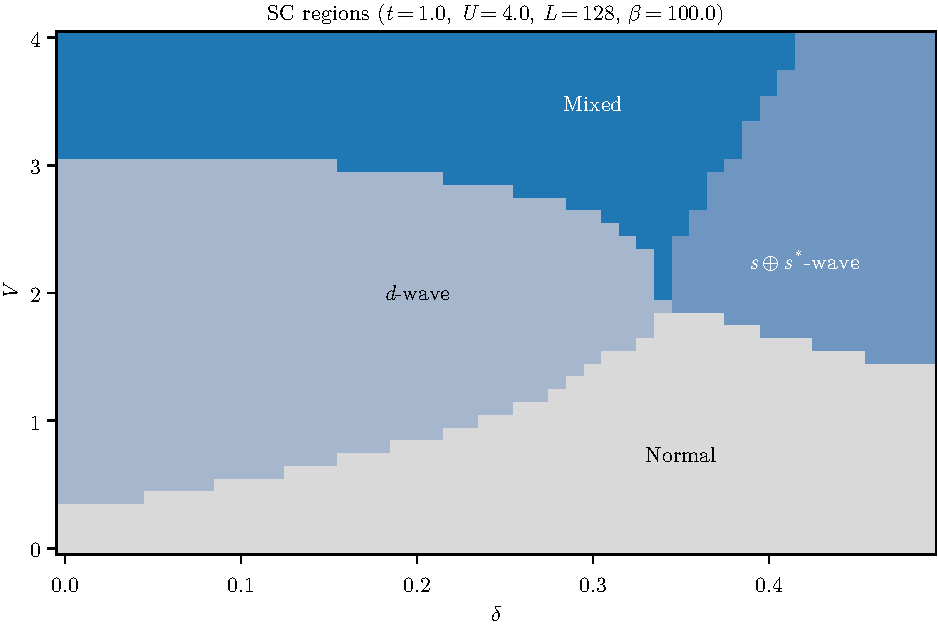
\includegraphics[height=0.32\linewidth]{../Project/src/labs/superconductor-boundary/w-U=4.0-solid.pdf}
		\label{subfig:sc-mix-U=4}
	}
	\subfloat[SC regions at $U=12.0$.]{
		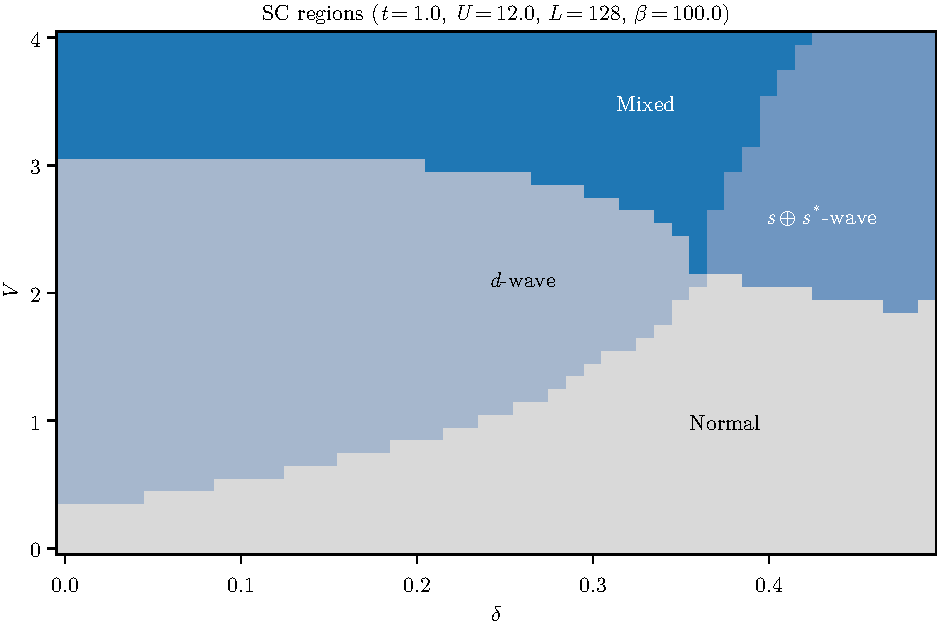
\includegraphics[height=0.32\linewidth]{../Project/src/labs/superconductor-boundary/w-U=12.0-solid.pdf}
		\label{subfig:sc-mix-U=12}
	}
	\caption{Depiction of the regions }
	\label{fig:sc-mix}
\end{figure}

In Fig.~\ref{fig:sc-mix} we see that mixing occurs at $V/t \approx 3$ at low doping, while increasing doping the boundary moves up. Therefore, a critical value of $V_\mathrm{c}[\delta]$ exists at each doping, above which superconductivity is established in singlet channel with a mixed topology. This leads us to the subject of next section. The most dramatic consequence of mixing is the breaking of planar rotational symmetry, namely,
\[
	\mathrm{C}_4 \SSB \mathrm{C}_2
\]

\subsection{Rotational SSB and nematic superconductivity}

\todo

\begin{figure}
	\centering
	\subfloat[Dependency of $t^{(s)}$ on $V$ at various $U$s, compared at three values of $\delta$.]{
		
\includegraphics[width=\linewidth]{/home/nepero27178/Thesis/EHM-HF/Project/plots/refined/Mode=hs/Phase=SC-Singlet/Setup=A[256]/Syms=Ssd/RB=Sd/Obj=RMPs/xVar=V_pVar=U/tS_t=1.0_L=256_δ=Compared_β=100.0.pdf}
		\label{subfig:sc-data-tS-A256-compared}
	}\\
	\subfloat[Dependency of $t^{(s)}$ on $\delta$ at various $V$s, compared at three values of $U$.]{
		
\includegraphics[width=\linewidth]{/home/nepero27178/Thesis/EHM-HF/Project/plots/refined/Mode=hs/Phase=SC-Singlet/Setup=B[256]/Syms=Ssd/RB=Sd/Obj=RMPs/xVar=δ_pVar=V/tS_t=1.0_U=Compared_L=256_β=100.0.pdf}
		\label{subfig:sc-data-tS-B256-compared}
	}
	\caption{Dependency of the $s^*$-wave renormalised hopping $t^{(s^*)}$ varying the doping $\delta$ and the local repulsion $U$. In the top panel we compare three doping levels $\delta=0.0,~0.2,~0.4$ varying $0 \le U \le 8$. In the bottom panel we compare three repulsion values $U=0.0,~5.0,~10.0$ varying $0 \le \delta \le 0.45$.}
	\label{fig:sc-data-tS-AB256-compared}
\end{figure}

\begin{figure}
	\centering
	\subfloat[Dependency of $t^{(d)}$ on $V$ at various $U$s, compared at three values of $\delta$.]{
		
\includegraphics[width=\linewidth]{/home/nepero27178/Thesis/EHM-HF/Project/plots/refined/Mode=hs/Phase=SC-Singlet/Setup=A[256]/Syms=Ssd/RB=Sd/Obj=RMPs/xVar=V_pVar=U/td_t=1.0_L=256_δ=Compared_β=100.0.pdf}
		\label{subfig:sc-data-td-A256-compared}
	}\\
	\subfloat[Dependency of $t^{(d)}$ on $\delta$ at various $V$s, compared at three values of $U$.]{
		
\includegraphics[width=\linewidth]{/home/nepero27178/Thesis/EHM-HF/Project/plots/refined/Mode=hs/Phase=SC-Singlet/Setup=B[256]/Syms=Ssd/RB=Sd/Obj=RMPs/xVar=δ_pVar=V/td_t=1.0_U=Compared_L=256_β=100.0.pdf}
		\label{subfig:sc-data-td-B256-compared}
	}
	\caption{Dependency of the $d$-wave renormalised hopping $t^{(d)}$ varying the doping $\delta$ and the local repulsion $U$. In the top panel we compare three doping levels $\delta=0.0,~0.2,~0.4$ varying $0 \le U \le 8$. In the bottom panel we compare three repulsion values $U=0.0,~5.0,~10.0$ varying $0 \le \delta \le 0.45$.}
	\label{fig:sc-data-td-AB256-compared}
\end{figure}

\begin{figure}
	\centering
	\subfloat[Nematic hopping at $U=4$.]{
		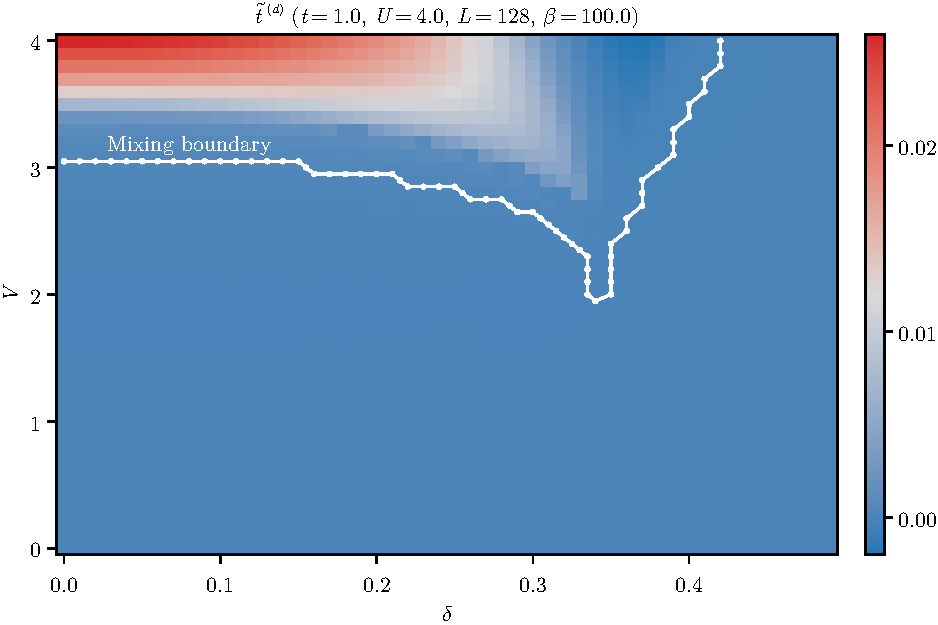
\includegraphics[height=0.32\linewidth]{../Project/src/labs/superconductor-boundary/w-U=4.0-curves.pdf}
		\label{subfig:sc-td-U=4}
	}
	\subfloat[Nematic hopping at $U=12$.]{
		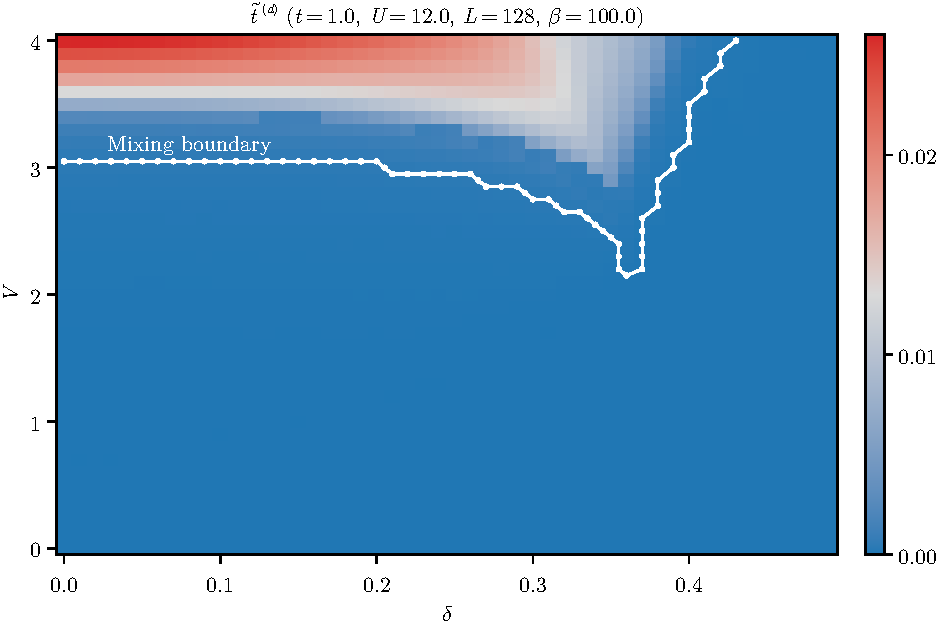
\includegraphics[height=0.32\linewidth]{../Project/src/labs/superconductor-boundary/w-U=12.0-curves.pdf}
		\label{subfig:sc-td-U=12}
	}
	\caption{}
	\label{fig:sc-td}
\end{figure}